\documentclass[12pt,a4paper,oneside]{report}             % Single-side
%\documentclass[11pt,a4paper,twoside,openright]{report}  % Duplex

\usepackage{ifxetex}
\ifxetex
  \usepackage{fontspec}
\else
  \usepackage[T1]{fontenc}
  \usepackage[utf8]{inputenc}
  \usepackage{lmodern}
\fi

\usepackage[magyar]{babel} % Alapértelmezés szerint utoljára definiált nyelv lesz aktív, de később külön beállítjuk az aktív nyelvet.

\usepackage{combelow}
\usepackage{newunicodechar}

\newunicodechar{Ș}{\cb{S}}
\newunicodechar{ș}{\cb{s}}
\newunicodechar{Ț}{\cb{T}}
\newunicodechar{ț}{\cb{t}}

\usepackage{cmap}
\usepackage{amsfonts,amsmath,amssymb} % Mathematical symbols.
\usepackage[ruled,boxed,resetcount,linesnumbered]{algorithm2e} % For pseudocodes.
\def\algorithmcfname{algoritmus}
\makeatletter
\renewcommand{\fnum@algocf}{\AlCapSty{\AlCapFnt\thealgocf.\nobreakspace\algorithmcfname}}
\makeatother

\usepackage{booktabs} % For publication quality tables for LaTeX
\usepackage{graphicx}
\usepackage{sidecap}

%\usepackage{fancyhdr}
%\usepackage{lastpage}

\usepackage{anysize}
\usepackage{sectsty}
\usepackage{setspace}  % Ettol a tablazatok, abrak, labjegyzetek maradnak 1-es sorkozzel!

% For hyperlinks in the generated document. 
\usepackage{color}
\usepackage{listings} % For source code snippets.

%\usepackage[amsmath,thmmarks]{ntheorem} % Theorem-like environments.

\usepackage[hang]{caption}
\usepackage{scrextend}

\usepackage{indentfirst}
\usepackage{pdfpages}

\usepackage{xfrac}
\usepackage{eurosym}

\usepackage{fullpage} % a margokra is lehessen irni

\newcommand{\vigyazat}{\marginpar{\textcolor{red}{\emph{Vigy\'azat!}}}}

\usepackage{tikz}
\usepackage{verbatim}
\usetikzlibrary{arrows,shapes}
\usetikzlibrary{positioning}
\tikzset{main node/.style={circle,fill=blue!20,draw,minimum size=1cm,inner sep=0pt},
}

%--------------------------------------------------------------------------------------
% Language configuration -- choose one
%--------------------------------------------------------------------------------------
\input{content/thesis-hu}  % Beállítások magyar nyelvű dolgozathoz

%--------------------------------------------------------------------------------------
% Main variables
%--------------------------------------------------------------------------------------



% Szak alapkepzes vagy mesteri
\newcommand{\szakHU}{INFORMATIKA SZAK} % SZOFTVERFEJLESZTES
\newcommand{\szakRO}{SPECIALIZAREA INFORMATIC\v A} % SPECIALIZAREA DEZVOLTAREA APLICA\c TIILOR SOFTWARE
\newcommand{\szakEN}{COMPUTER SCIENCE SPECIALIZATION} %SOFTWARE DEVELOPMENT SPECIALIZATION


\newcommand{\dolgozattipusHU}{DIPLOMADOLGOZAT} % MESTERI DISSZERT\'ACI\'O
\newcommand{\dolgozattipusRO}{LUCRARE DE DIPLOM\v A} %TEZA DE MASTERAT
\newcommand{\dolgozattipusEN}{BACHELOR THESIS} % MASTER THESIS

\newcommand{\szerzo}{Kovács Bence} % Szerző neve
\newcommand{\temavezetoA}{Dr. Márton Gyöngyvér} 


% Fokozatok

%Egyetemi tan\'ar/ Profesor universitar/Full Professor
%Egyetemi docens/ Conferențiar universitar/Associate professor
%Egyetemi adjunktus/Lector universitar sau Șef de lucrări /Lecturer
%Egyetemi tan\'arseg\'ed/Asistent universitar/Assistant professor


\newcommand{\temavezetoAfokozat}{Egyetemi adjunktus}% Első konzulens neve
\newcommand{\temavezetoAfokozatRo}{Șef de lucrări}
\newcommand{\temavezetoAfokozatEn}{Lecturer}
\newcommand{\temavezetoB}{Györfi Ágnes} % Második konzulens neve; hagyd üresen, ha egy konzulensed van.
\newcommand{\temavezetoBfokozat}{Egyetemi tan\'arseg\'ed}
\newcommand{\temavezetoBfokozatRo}{Asistent universitar}
\newcommand{\temavezetoBfokozatEn}{Assistant professor}
\newcommand{\cimHu}{F1 Ticket Manager - Online jegyek kezelése} % Cím
\newcommand{\cimRO}{F1 Ticket Manager - Gestiunea tichetelor}
\newcommand{\cimEN}{F1 Ticket Manager - Online ticket management}
\newcommand{\ev}{2023} %az aktualis ev

%--------------------------------------------------------------------------------------
% Page layout setup
%--------------------------------------------------------------------------------------
% we need to redefine the pagestyle plain
% another possibility is to use the body of this command without \fancypagestyle
% and use \pagestyle{fancy} but in that case the special pages
% (like the ToC, the References, and the Chapter pages)remain in plane style

\usepackage{smartdiagram}
\usepackage{tikz,pgf}
\usepackage{pgfplots}
\pgfplotsset{width=7cm,compat=1.8}
\usetikzlibrary{matrix,calc,shapes}

\tikzset{
	treenode/.style = {shape=rectangle, rounded corners, draw, anchor=center, text width=5em, align=center, top color=white, bottom color=blue!20,inner sep=1ex},
	decision/.style = {treenode, diamond, inner sep=0pt},
	root/.style = {treenode, font=\Large, bottom color=red!30},
	env/.style = {treenode, font=\ttfamily\normalsize},
	finish/.style = {root, bottom color=green!40},
	dummy/.style = {circle,draw}
}


\setcounter{secnumdepth}{0}
\sectionfont{\large\upshape\bfseries}
\setcounter{secnumdepth}{2}

\sloppy % Margón túllógó sorok tiltása.
\widowpenalty=10000 \clubpenalty=10000 %A fattyú- és árvasorok elkerülése
\def\hyph{-\penalty0\hskip0pt\relax} % Kötőjeles szavak elválasztásának engedélyezése


%--------------------------------------------------------------------------------------
% Setup hyperref package
%--------------------------------------------------------------------------------------
\usepackage{xcolor}
\definecolor{bluecite}{HTML}{0875b7}
\usepackage[unicode=true,
bookmarksopen={true},
pdffitwindow=true, 
colorlinks=true, 
linkcolor=bluecite, 
citecolor=bluecite, 
urlcolor=bluecite, 
hyperfootnotes=false, 
pdfstartview={FitH},
pdfpagemode= UseNone]{hyperref}


%--------------------------------------------------------------------------------------
% Set up listings
%--------------------------------------------------------------------------------------



\definecolor{codegreen}{rgb}{0,0.6,0}
\definecolor{codegray}{rgb}{0.5,0.5,0.5}
\definecolor{codepurple}{rgb}{0.58,0,0.82}
\definecolor{backcolour}{rgb}{0.95,0.95,0.92}




\definecolor{lightgray}{rgb}{0.95,0.95,0.95}
\definecolor{darkgreen}{RGB}{3,125,80}
\lstset{frame=tb,
	language=Matlab,
	aboveskip=3mm,
	belowskip=3mm,
	showstringspaces=false,
	columns=flexible,
	basicstyle={\small\ttfamily},
	numbers=none,
	numberstyle=\tiny\color{gray},
	keywordstyle=\color{blue},
	commentstyle=\color{codegreen},
	%stringstyle=\color{mauve},
	breaklines=true,
	breakatwhitespace=true,
	tabsize=3,
	backgroundcolor=\color{lightgray},
}
\def\lstlistingname{k\'odr\'eszlet}	


%--------------------------------------------------------------------------------------
% Set up theorem-like environments
%--------------------------------------------------------------------------------------
% Using ntheorem package -- see http://www.math.washington.edu/tex-archive/macros/latex/contrib/ntheorem/ntheorem.pdf
%\swapnumbers
%\theoremstyle{plain}
%\theoremseparator{.}
\newtheorem{example}{\pelda}[section]

%\theoremseparator{.}
%\theoremprework{\bigskip\hrule\medskip}
%\theorempostwork{\hrule\bigskip}
%\theorembodyfont{\upshape}
%\theoremsymbol{{\large \ensuremath{\centerdot}}}
\newtheorem{definition}{\definicio}[section]

%\theoremseparator{.}
%\theoremprework{\bigskip\hrule\medskip}
%\theorempostwork{\hrule\bigskip}
\newtheorem{theorem}{\tetel}[section]

\newtheorem{conclusion}{Következtetés}[section]


%--------------------------------------------------------------------------------------
% Some new commands and declarations
%--------------------------------------------------------------------------------------
\newcommand{\code}[1]{{\upshape\ttfamily\scriptsize\indent #1}}
\newcommand{\doi}[1]{DOI: \href{http://dx.doi.org/\detokenize{#1}}{\raggedright{\texttt{\detokenize{#1}}}}} % A hivatkozások közt így könnyebb DOI-t megadni.

\DeclareMathOperator*{\argmax}{arg\,max}
%\DeclareMathOperator*[1]{\floor}{arg\,max}
\DeclareMathOperator{\sign}{sgn}
\DeclareMathOperator{\rot}{rot}


%--------------------------------------------------------------------------------------
% Setup captions
%--------------------------------------------------------------------------------------

\captionsetup[figure]{
	width=.75\textwidth,
	aboveskip=10pt}
\renewcommand{\captionlabelfont}{\bf}
%\renewcommand{\captionfont}{\footnotesize\it}


%--------------------------------------------------------------------------------------
% Redefine reference style
%--------------------------------------------------------------------------------------
\newcommand{\figref}[1]{\ref{fig:#1}.}
\renewcommand{\eqref}[1]{(\ref{eq:#1})}
\newcommand{\listref}[1]{\ref{listing:#1}.}
\newcommand{\sectref}[1]{\ref{sect:#1}}
\newcommand{\tabref}[1]{\ref{tab:#1}.}





%--------------------------------------------------------------------------------------
% Table of contents and the main text
%--------------------------------------------------------------------------------------
\begin{document}

% CIMOLDALAK
%~~~~~~~~~~~~~~~~~~~~~~~~~~~~~~~~~~~~~~~~~~~~~~~~~~~~~~~~~~~~~~~~~~~~~~~~~~~~~~~~~~~~~~
	%--------------------------------------------------------------------------------------
%	A magyar cimoldal
%--------------------------------------------------------------------------------------
\begin{titlepage}
	\begin{center}
	
		\large{\bfseries SAPIENTIA ERDÉLYI MAGYAR TUDOMÁNYEGYETEM} \\
		\large{\bfseries MAROSVÁSÁRHELYI KAR,} \\
		\large{\bfseries \szakHU} \\[2.5cm]
			\begin{center}
			\includegraphics[scale=2]{images/sapientia-hu}
		\end{center}
		\vspace{0.4cm}
		\Large{\Large  \cimHu}\\[0.8cm]
		\vspace{0.2cm}
		\textsc{\Large \bfseries \dolgozattipusHU}\\[2.5cm]
		
		{
			\large
		
			\renewcommand{\arraystretch}{0.85}
			\begin{tabular}{cc}
				  \makebox[6.5cm]{Témavezető:} & \makebox[6.5cm]{Végzős hallgató:} \\ \noalign{\smallskip}
				  \makebox[6.5cm]{\temavezetoA,} & \makebox[6.5cm]{\szerzo} \\ {\temavezetoAfokozat} \\
				  \makebox[6.5cm]{\temavezetoB,} & \\ {\temavezetoBfokozat} \\
			\end{tabular}
		}
		
		\vfill
		{\large \bfseries \ev}
	\end{center}
\end{titlepage}
	%--------------------------------------------------------------------------------------
%	The title page RO
%--------------------------------------------------------------------------------------

\begin{titlepage}
	\begin{center}
	
		\large{\bfseries UNIVERSITATEA SAPIENTIA DIN CLUJ-NAPOCA} \\
		\large{\bfseries FACULTATEA DE ȘTIINȚE TEHNICE ȘI UMANISTE,} \\
		
		\large{\bfseries \szakRO} \\[2.5cm]
		
			\begin{center}
			\includegraphics[scale=2]{images/sapientia-ro}
		\end{center}
		
		\vspace{0.4cm}
		
	
		
		\Large{\Large \cimRO}\\[0.8cm]
		\vspace{0.5cm}
		\textsc{\Large \bfseries \dolgozattipusRO}\\[2.5cm]
		
		{
			\large
		
			\renewcommand{\arraystretch}{0.85}
			\begin{tabular}{cc}
				 \makebox[6.5cm]{Coordonator științific:} & \makebox[6.5cm]{Absolvent:} \\ \noalign{\smallskip}
				 \makebox[6.5cm]{\temavezetoA,} & \makebox[6.5cm]{\szerzo} \\
				 {\temavezetoAfokozatRo}
			\end{tabular}
		}
		
		\vfill
		{\large \bfseries \ev}
	\end{center}
\end{titlepage}
	%--------------------------------------------------------------------------------------
%	The title page EN
%--------------------------------------------------------------------------------------

\begin{titlepage}
	\begin{center}
	
		\large{\bfseries SAPIENTIA HUNGARIAN UNIVERSITY OF TRANSYLVANIA} \\
		\large{\bfseries FACULTY OF TECHNICAL AND HUMAN SCIENCES} \\
		\large{\bfseries \szakEN} \\[2.5cm]
		
			\begin{center}
			\includegraphics[scale=2]{images/sapientia-en}
		\end{center}
		\vspace{0.4cm}
		\Large{\Large  \cimEN}\\[0.8cm]
		\vspace{0.5cm}
		\textsc{\Large \bfseries \dolgozattipusEN}\\[2.5cm]
		
		{
			\large
	
			\renewcommand{\arraystretch}{0.85}
			\begin{tabular}{cc}
				 \makebox[6.5cm]{Scientific advisor:} & \makebox[6.5cm]{Student:} \\ \noalign{\smallskip}
				 \makebox[6.5cm]{\temavezetoA,} & \makebox[6.5cm]{\szerzo} \\
				 {\temavezetoAfokozatEn}
			\end{tabular}
		}
		
		\vfill
		{\large \bfseries \ev}
	\end{center}
\end{titlepage}
	
	\includepdf[pages={1}]{content/Fisa-proiectului.pdf}
	\includepdf[pages={1}]{content/Declaratie.pdf}

	\pagenumbering{gobble}

\selectlanguage{magyar}
\hungarianParagraph

%----------------------------------------------------------------------------
% Abstract in Hungarian
%----------------------------------------------------------------------------

\chapter*{Kivonat}

Napjainkban az online jegyvásárlás rohamos elterjedése figyelhető meg a technológia fejlődésével és az internet elérhetőségének növekedésével. Egy online platformon keresztül az emberek ma már kényelmesen és gyorsan tudnak jegyeket vásárolni különféle eseményekre, mint például koncertekre, színházi előadásokra vagy sporteseményekre, mint például a Formula-1.

Az online jegyvásárlás számos előnnyel jár. A vásárlók egyszerűen és kényelmesen böngészhetnek és választhatnak a széles körű jegyválaszték közül. Az online platformok részletes információkat nyújtanak az eseményekről, beleértve a dátumokat, helyszíneket és leírásokat. Emellett az online jegyvásárlás lehetővé teszi a jegyek összehasonlítását, árak és típusok kiválasztását, ami segít a vásárlóknak a legjobb lehetőség megtalálásában.

A technológiai fejlesztések, mint például a biztonságos online fizetési rendszerek és az elektronikus jegyek, hozzájárultak az online jegyvásárlás elterjedéséhez. A vásárlók könnyedén és biztonságosan fizethetnek az online platformokon (webshop) keresztül, és elektronikus jegyet kapnak, amelyet mobil eszközükön vagy nyomtatható formában mutathatnak fel az eseményen. Az online jegyvásárlás megkönnyíti az eseményekre való részvételt, hiszen a vásárlóknak nem kell hosszú sorokban állniuk a jegypénztáraknál. 


\vfill
\selectlanguage{romanian}

%----------------------------------------------------------------------------
% Abstract in Romanian
%----------------------------------------------------------------------------
\chapter*{Rezumat}

În prezent, se observă o răspândire rapidă a achiziționării de bilete online, odată cu dezvoltarea tehnologică și creșterea accesului la internet. Prin intermediul unei platforme online, oamenii pot cumpăra bilete confortabil și rapid pentru diverse evenimente, cum ar fi concerte, spectacole de teatru sau evenimente sportive, precum Formula 1.

Achiziționarea de bilete online vine cu numeroase avantaje. Cumpărătorii pot naviga și alege cu ușurință dintr-o gamă largă de opțiuni de bilete. Platformele online oferă informații detaliate despre evenimente, inclusiv date, locații și descrieri. De asemenea, achiziționarea de bilete online permite compararea prețurilor și selecționarea diferitelor tipuri de bilete, ceea ce ajută cumpărătorii să găsească cea mai bună opțiune.

Dezvoltările tehnologice, cum ar fi sistemele de plată online sigure și biletele electronice, au contribuit la răspândirea achiziționării de bilete online. Cumpărătorii pot plăti ușor și în siguranță prin intermediul platformelor online (webshop) și primesc biletele electronice, pe care le pot prezenta pe dispozitivele lor mobile sau sub formă printată la eveniment. Achiziționarea de bilete online facilitează participarea la evenimente, deoarece cumpărătorii nu mai trebuie să stea în rânduri lungi la casele de bilete.


\vfill
\selectlanguage{english}
%\englishParagraph

%----------------------------------------------------------------------------
% Abstract in English
%----------------------------------------------------------------------------
\chapter*{Abstract}

Currently, the rapid spread of online ticket purchasing can be observed due to technological advancements and the increased accessibility of the internet. Through an online platform, people can now conveniently and quickly purchase tickets for various events such as concerts, theater performances, or sports events like Formula 1.

Online ticket purchasing comes with numerous advantages. Customers can easily browse and choose from a wide range of ticket options. Online platforms provide detailed information about events, including dates, venues, and descriptions. Additionally, online ticket purchasing allows for ticket comparisons, price and type selections, which help customers find the best options available.

Technological developments, such as secure online payment systems and electronic tickets, have contributed to the widespread adoption of online ticket purchasing. Customers can easily and safely make payments through online platforms (webshop) and receive electronic tickets that can be presented on their mobile devices or in printable form at the event. Online ticket purchasing simplifies event attendance, as customers no longer have to wait in long queues at ticket counters.


\vfill
\dolgozatnyelve
\defaultParagraph
 
% Tartalomjegyzek
%~~~~~~~~~~~~~~~~~~~~~~~~~~~~~~~~~~~~~~~~~~~~~~~~~~~~~~~~~~~~~~~~~~~~~~~~~~~~~~~~~~~~~~
	\pagenumbering{arabic}
	\setcounter{page}{9}
	\tableofcontents\vfill

% A diplomadolgozat lenyegi resze
%~~~~~~~~~~~~~~~~~~~~~~~~~~~~~~~~~~~~~~~~~~~~~~~~~~~~~~~~~~~~~~~~~~~~~~~~~~~~~~~~~~~~~~

% ajánlott külön file-okba írni az egyes fejezeteket, ugyanis úgy jobban át lehet látni.

	

	%----------------------------------------------------------------------------
\chapter{Bevezető}%\addcontentsline{toc}{chapter}{Bevezető}
%----------------------------------------------------------------------------

\lstdefinelanguage{JavaScript}{
  keywords={
    typeof, new, true, false, catch, function, return, null, catch, switch, var,
    if, in, while, do, else, case, break, export, import
  },
  keywordstyle=\color{blue}\bfseries,
  ndkeywords={
    class, extends, const, let, constructor, super, static
  },
  ndkeywordstyle=\color{purple}\bfseries,
  identifierstyle=\color{black},
  sensitive=false,
  comment=[l]{//},
  morecomment=[s]{/*}{*/},
  commentstyle=\color{green}\ttfamily,
  stringstyle=\color{red}\ttfamily,
  morestring=[b]',
  morestring=[b]",
  literate=
    *{0}{{\textcolor{blue}{0}}}{1}
    {1}{{\textcolor{blue}{1}}}{1}
    {2}{{\textcolor{blue}{2}}}{1}
    {3}{{\textcolor{blue}{3}}}{1}
    {4}{{\textcolor{blue}{4}}}{1}
    {5}{{\textcolor{blue}{5}}}{1}
    {6}{{\textcolor{blue}{6}}}{1}
    {7}{{\textcolor{blue}{7}}}{1}
    {8}{{\textcolor{blue}{8}}}{1}
    {9}{{\textcolor{blue}{9}}}{1}
    {\ }{{ }}{1},
  keywords=[2]{random, PBKDF2, toString, stringify, encrypt},
  keywordstyle=[2]\color{green}\bfseries
}

\section {Témaválasztás indoklása}

Napjainkban az online jegyvásárlás nagy előretörést ért el a technológia fejlődésével az egyre szélesebb körben történő bankkártyás internetes vásárlások következtében. Egy online platformon keresztül az emberek ma már kényelmesen és gyorsan tudnak jegyeket vásárolni különféle eseményekre tekintettel arra, hogy percek alatt el tudjuk végezni a világ bármely pontjából a nap bármely időpontjában. Az online jegyvásárlás számos előnnyel jár, amelyeknek köszönhetően egyre népszerűbbé válik.

Az egyik legfontosabb előny az online jegyvásárlás esetén az, hogy a vásárlók egyszerűen és kényelmesen böngészhetnek és választhatnak a széles körű jegyválaszték közül. Az online platformok részletes információkat biztosítanak az eseményekről, így a potenciális vásárlók teljes körű tájékoztatást kapnak az eseményről, mielőtt eldöntenék, hogy vásárolnak-e jegyet. Tehát a vásárlók magabiztosan dönthetnek arról, hogy melyik eseményre szeretnének jegyet vásárolni, anélkül, hogy bármilyen korlátozásba ütköznének.

A technológiai fejlesztések, mint például a biztonságos online fizetési rendszerek (\ref{abra:Logok}), amelyek az EDI rendszerek alkomponenseként ismert, és az elektronikus jegyek, hozzájárultak az online jegyvásárlás népszerűségéhez. A vásárlók könnyedén és biztonságosan fizethetnek az online platformokon keresztül, és elektronikus jegyet kapnak, amelyet mobil eszközükön vagy nyomtatható formában mutathatnak fel az eseményen. Az elektronikus jegyek további előnye, hogy nehezen veszíthetőek el vagy semmisülhetnek meg, így a vásárlók biztonságban tudhatják az értékes jegyeiket. Itt fontos megemlíteni, hogy ezen jegyek tárolása és biztonságban tartása további adatbiztonsági kérdéseket vet fel, amellyel foglalkozunk a dolgozat keretében. A platformokon keresztül a vásárlók egyszerűen választhatják ki a kívánt eseményt, a megfelelő ülőhelyet vagy jegytípust, és azonnal megvásárolhatják a jegyüket néhány kattintással. Ez időt és energiát takarít meg a vásárlók számára, ami napjainkban egy lényeges tényező.

\begin{figure}[!h]
	\centering
	\includegraphics[scale=0.2]{images/logok}
	\caption{Online fizetési rendszerek}
	\label{abra:Logok}
\end{figure}
\pagebreak

További előnyeként egy ilyen platformnak megemlítendő, hogy a szervezők számára is jelentősen hatékonyabbá teszi a rendelések nyomon követését, statisztikák készítését, amelyeket felhasználhatnak értékesítési jelentések és a marketing javításához. Emellett az online jegyvásárlás lehetőséget nyújt a szervezőknek arra is, hogy célzottan reklámozzák az eseményüket, így nagyobb látogatottságot érhetnek el.

A jelenleg is működő hivatalos platform, ahol direkt módon juthatunk hozzá jegyekhez az F1-es versenyhétvégékre, az F1 Experiences. Itt gyorsan és kényelmesen vásárolhatjuk meg a kívánt jegyünket, amelyet a sikeres rendelés és kifizetés után emailben kapjuk meg PDF formátumban, amely tartalmazza a megvásárolt jegy(ek)et, egyedi azonosítókat és QR kódokat. Az email továbbá tartalmazza a számlázási adatokat. Az eseményre érve, a belépő kapuknál, egy erre a célra kihelyezett okos eszközzel megtörténik a QR kód olvasása és hitelesítése. Pozitív eredmény esetén beléphetünk az esemény helyszínére.

A fent említett folyamat megengedi, hogy ezek az elektronikus jegyek átruházhatóak a tulajdonos által bárki számára. Ezzel persze önmagában nincs probléma, mivel ezt a szabadságot meg kell lehessen adni a felhasználóknak, hogy bizonyos esetekben más személy tudjon részt venni a vásárló helyett, így nem veszik kárba a vásárlás. Ez a rendszer viszont teret ad egy olyan biztonsági kérdésnek, amelyet jelenleg a felhasználó felelősségére van bízva, miszerint ezt a kódot akár hetekkel, hónapokkal a használatuk előtt kapnak meg a felhasználók elektronikus levél formájában és azt bárki megszerezheti, akinek hozzáférése van a fiókhoz. Rosszabb esetekben, egy szándékos kibernetikai támadás esetén is eltulajdoníthatják és felhasználhatják. Ennek persze kisebb a valószínűsége, viszont ami egy aggasztó tény, hogy a felhasználók nagy része nem megfelelő módon kezeli az adatainak a biztonságos tárolását és számos esetben fellelhetőek olyan emberi hibák, amelyeket kihasználnak az adathalászok, hogy hozzáférjenek a megvásárolt jegyekhez és saját célokra használják fel, többnyire illegális módon kereskedni velük.

Gyakran megtörténik, hogy egy felhasználó több oldalra is ugyan azokat a bejelentkezési adatokat adja meg a regisztráció során. Ez többségében a személyes email fiók felhasználó nevével és jelszójával megegyezik és ezt az adathalászok is figyelembe veszik. Egy másik sebezhetőség, hogy számos esetben egy fiókhoz több személy is hozzáfér, így már nem beszélhetünk biztonságos adattárolásról. Megemlítendő viszont, hogy az email szolgáltatók biztosítanak E2EE-t az elektronikus levelek küldésekor és fogadásakor.

Az F1 Ticket Manager webes alkalmazás célja az alapvető jegyvásárlási funkcionalitások biztosítása, valamint a teljes vásárlási folyamat biztonságosabbá tétele. Ennek megvalósítására számos technológiai fejlesztés és programozói technika létezik. Az alkalmazás fejlesztésénél beépítésre került PIN kódok használata, amely egy emelt szintű biztonságot nyújt a felhasználó számára, valamint EGY? titkosítási algoritmus, amely az eredeti adatok azonnali visszafejtését hivatott megnehezíteni. 

\section {Elméleti megalapozás és szakirodalmi áttekintő}
\subsection {Webes alkalamazás felépítése}

Az F1TM a React JavaScript programozási nyelv keretrendszerével valósult meg a Microsoft Visual Studio Code IDE-ben. Az alkalmazás használ harmadik féltől származó könyvtárakat is, amelyek felgyorsítják a fejlesztési folyamatot, mivel előre le van implementálva számos funkcionalitás. Ezek általában több fejlesztő által használtak és vannak tesztelve, ezért többségében gyorsabbak és biztonságosabbak.

Lévén, hogy az alkalmazás egy webes platform, a struktúrája két fő részből áll: frontend és backend. Ezen projekt keretében első sorban a frontend implementációján volt a hangsúly.

A frontend az a része a webes alkalmazásnak, amellyel a felhasználók közvetlenül interakcióba lépnek. Ez a rész felelős a UI megjelenítéséért és a felhasználói interakciók kezeléséért. A frontend általában a böngészőben fut, és a felhasználó által látott elemeket jeleníti meg, például az oldalak, űrlapok, gombok, navigációs elemek stb. A frontend tervezésekor figyelembe kell venni a UX aspektusait is. Ezek azért felelnek, hogy a felhasználói élmény a lehető legjobb legyen a weboldal böngészése során. Itt első sorban a letisztultság, átláthatóság és az összezavaró elemek elkerülése a legfőbb cél.

A frontend technológiák közé tartozhatnak:
\begin{itemize}
	\item HTML: Az alapvető struktúrát és tartalmat határozza meg a weboldalakhoz.
	\item CSS: A megjelenítést és a stílust adja a weboldalaknak, mint például a színek, betűtípusok, elrendezés stb.
	\item JavaScript: A dinamikus és interaktív funkciókért felelős, például animációk, eseménykezelés, adatmanipuláció. Gyakran használnak frontend keretrendszereket, például a React JS-t, Next.js-t vagy Angular-t, amelyek segítenek az alkalmazás fejlesztésében és szervezésében. 
\end{itemize}

A backend a szerveroldali logikát és adatkezelést végzi. Ez a rész felelős az adatbáziskezelésért, a logika végrehajtásáért, a felhasználói kérések feldolgozásáért és a válaszok generálásáért. A backend nem közvetlenül látható vagy interaktív a felhasználók számára, viszont folyamatosan kommunikál a frontend-el az API-kon keresztül.

A backend technológiák közé tartozhatnak:
\begin{itemize}
	\item Szerveroldali programozási nyelvek: Python, Ruby, Java, PHP stb.
	\item Keretrendszerek: Node.js, Django, Ruby on Rails, Laravel stb., amelyek segítenek az alkalmazás fejlesztésében és a szerveroldali logika megvalósításában.
	\item Adatbázis-kezelő rendszerek: MySQL, PostgreSQL, MongoDB stb., amelyek tárolják az alkalmazás adatai és lehetővé teszik ezek lekérdezését és manipulálását.
\end{itemize}

A frontend és backend között kommunikáció történik HTTP kérések és válaszok segítségével. A frontend kéréseket küld a backendnek, például adatlekérdezések vagy műveletek végrehajtása érdekében. Ezek a backend(ek) API végpontjain keresztül történnek A backend feldolgozza ezeket a kéréseket, és visszaküldi a válaszokat a frontendnek (\ref{abra:Architektura}). Nagyon alkalmazások esetében megtörténhet, hogy a frontend több backend szerverről kéri le az információkat. Ez az felhasználó számára nem feltűnő, mivel egy megfelelő UX-szel rendelkező frontend minden esetben egy státuszjelző elemet helyez a betöltés idejére (animáció), függetlenül attól, hogy éppen melyik szerverrel történik a kommunikáció.

\begin{figure}[!h]
	\centering
	\includegraphics[scale=0.2]{images/architektura}
	\caption{Webes alkalmazás architekúrája}
	\label{abra:Architektura}
\end{figure}

\subsection {A React JavaScript keretrendszer}

Az elmúlt években a React JS jelentős népszerűségre tett szert a webfejlesztés területén. A React egy nyílt forráskódú JavaScript keretrendszer, amelyet a Facebook (Meta) fejlesztett ki, és célja a felhasználói felületek könnyű és hatékony megvalósítása. A React alapvetően egy komponens alapú megközelítést kínál, amely lehetővé teszi a fejlesztők számára, hogy újra felhasználható, önálló építőelemeket hozzanak létre, amelyeket könnyedén kombinálhatnak egymással a komplexebb felhasználói felületek elkészítése érdekében.

A React (\ref{abra:reactLogo}) rendkívül népszerűvé vált a fejlesztők körében számos előnye miatt. Elsőként említhetjük a hatékony Virtual DOM implementációját, amely lehetővé teszi az alkalmazások gyors és hatékony frissítését. A Virtual DOM a weboldal megjelenítéséhez használt valós DOM virtuális reprezentációja. Amikor változás történik az adatokban, a React a Virtual DOM-on keresztül kiszámítja az optimális frissítéseket, majd ezeket a változtatásokat csak a valós DOM-ra alkalmazza. Ez a megközelítés jelentős sebességjavulást eredményez a webalkalmazásokban.

A második fontos előny a komponens alapú megközelítés, amely lehetővé teszi a fejlesztők számára a komponensek újra felhasználását és a kód modularizációját. A React komponensek önmagukban zárt egységek, amelyek különböző feladatokat elláthatnak a felhasználói felületeken, például gombok, űrlapok, listák stb. Az egyedi komponensek könnyedén kombinálhatók egymással, így a fejlesztőknek nem kell újra megírniuk a kódot, hanem egyszerűen felhasználhatják a meglévő komponenseket.

Emellett más technológiai óriások is felfedezték a React előnyeit. Például a Netflix, a PayPal, az Airbnb és a Dropbox is a React-et használja az alkalmazásaik fejlesztéséhez. Ezek a vállalatok magas forgalommal és komplex felhasználói felületekkel rendelkeznek, és a React segítségével könnyedén kezelhetik ezeket a kihívásokat.

Az open-source software (OSS) közösség is hozzájárult a React népszerűségének növekedéséhez. Számos harmadik által (Third party) fél készített könyvtár és eszköz érhető el a React-hez, amelyek további lehetőségeket kínálnak a fejlesztőknek. Ilyen példa a Redux, amely egy állapotkezelő könyvtár, vagy a React Router, amely segít az alkalmazások útvonalainak kezelésében.

A JavaScript önmagában egy típusfüggetlen programozási nyelv, de egyes keretrendszerek, mint a Next.js, a Microsoft által kifejlesztett TypeScript nyelvet használják, amely már megengedi a beépített és személyre szabott típusok használatát.

\begin{figure}[!h]
	\centering
	\includegraphics[scale=0.04]{images/reactLogo}
	\caption{React logó}
	\label{abra:reactLogo}
\end{figure}

\subsection {A Google Firebase platform}

Mivel a React a webes alkalmazások frontend-jének fejlesztésére szolgál, szükségem volt egy backend szerverre és egy DBMS, -re, amely kiszolgálja a frontend-et, a Google által fejlesztett Firebase platformot és API-kat építettem be az alkalmazásba.
A Google Firebase (\ref{abra:firebaseLogo}) egy teljes körű fejlesztői platform, amely különféle eszközöket és szolgáltatásokat kínál a fejlesztőknek, hogy könnyedén hozzanak létre, teszteljenek és üzemeltessenek webes és mobilalkalmazásokat.

A Firebase Realtime Database egy NoSQL alapú adatbázis, amely valós idejű adatszinkronizációt tesz lehetővé az alkalmazások között. Ez azt jelenti, hogy az adatok automatikusan frissülnek minden csatlakozott eszközön, így a felhasználók valós idejű élményt élvezhetnek. Ez különösen hasznos például csevegőalkalmazások vagy valós idejű játékok fejlesztésekor. 

A Firebase Authentication lehetővé teszi a felhasználók egyszerű és biztonságos hitelesítését. Támogatja az e-mail és jelszó, a szociális média hitelesítés (pl. Google, Facebook, Twitter) és más autentikációs módokat is. A Firebase emellett lehetőséget biztosít a felhasználói fiókok-, profilok kezelésére és jogosultságkezelésre is. 

A Firebase Cloud Storage segítségével könnyedén tárolhatóak és kezelhetőek az alkalmazásban használt fájlok, például képek, hangfájlok vagy videók. Az egyszerű API-k lehetővé teszik a fájlok feltöltését, letöltését és megosztását. Emellett a Firebase Hosting segítségével egyszerűen és gyorsan kiszolgálhatod az alkalmazásod statikus fájljait a világ minden tájáról.

A Storage Bucket-ek egy nagy tárolóhelyet jelentenek a fájlok (például képek, hangfájlok, videók stb.) biztonságos tárolására a felhőben. A Firebase Storage lehetővé teszi a fájlok feltöltését, letöltését, törlését és megosztását egyszerű API-k segítségével. Emellett automatikusan kezeli a fájlok hozzáférési jogosultságait és a CDN révén biztosítja a gyors és megbízható fájlletöltést a felhasználóknak.

\begin{figure}[!h]
	\centering
	\includegraphics[scale=0.2]{images/firebaseLogo}
	\caption{Firebase logó}
	\label{abra:firebaseLogo}
\end{figure}

\section {Az AES titkosítás}
\subsection {Bevezető}

Az AES egy blokk titkosítási algoritmus, amelyet két belga kriptográfus tervezett 1997-ben. Az algoritmus az 1990-ben meghirdetett nyilvános pályázat nyertese lett, és 2001-ben a NIST (National Institute of Standards and Technology) elfogadta az Egyesült Államok kormányzati szervezetei számára ajánlott titkosítási szabványnak. Mivel az említett pályázat elbírálása publikusan történt, ezért valószínűleg nem történt befolyás a díj megítélését illetően. Az algoritmus egy változata a Rinjdael algoritmusnak, amely eredetileg több blokkmérettel is dolgozott és ebből választották ki az AES-t, amelynek blokkmérete 128 bit.

Az AES blokk mérete 128 bit, és a kulcs mérete lehet 128, 192 vagy 256 bit. Az AES hatékonysága körülbelül 109 Mb/s, amely természetesen függ az adott hardver tulajdonságaitól, és szakértők szerint a 256 bites kulcsméret biztonsága "örök" időkre szól.

Az AES nem használja a Feistel-sémát, mint a DES (Data Encryption Standard), hanem iteratív szerkezetű. Az algoritmus a kulcsméret alapján különböző számú körökben végzi a titkosítást, amelyekhez korkulcsokat generál. A 128 bites kulcs esetén a körök száma 10, a 192 bites kulcs esetén a körök száma 12, míg a 256 bites kulcs esetén a körök száma 14.

Az AES helyettesítést és permutációt alkalmaz a blokkon belül, és véges testek felett végez aritmetikai és műveletet. Az algoritmus térnyerésére az szolgált, hogy a művelet végzés egész számokkal történik, ezért a szerzők egy olyan algoritmust fejlesztettek, ahol az összeadás, kivonás, szorzás, osztás után is halmaz béli elemet kapunk. Az AES véges testként használja a bináris együtthatós polinomokat a GF(2\textasciicircum n) felett, ahol n = 8 fokszámnál kisebb.

Az AES minden műveletet 8 biten végez, és az összes 30 irreducibilis polinom közül a következőt használja: $x\textasciicircum 8 + x\textasciicircum 4 + x\textasciicircum 3 + x + 1$. Az AES minden bájtot a $GF(2\textasciicircum 8) = GF(2)[x]/(x\textasciicircum 8 + x\textasciicircum 4 + x\textasciicircum 3 + x + 1)$ testelemeként kezel.

Az AES-t általában három algoritmus alkotja: a kulcsgenerálás, a titkosítás és a visszafejtés. Az AES a bemeneti 128 bites állapotot (state) egy 4x4-es mátrix formájában kezeli, és az algoritmus minden iterációja során helyettesítő és permutációs műveleteket végez el a blokkon belül.

\subsection {Az algoritmus elmélete}

Az AES a bemeneti adatokat 128 bites blokkokra bontja. A bemeneti adatokat több körön keresztül módosítja míg el nem jutunk a titkosított adatig. A módosításokat az algoritmus több lépésben hajtja végre. Ezeket a lépéseket altranszformációknak nevezzük.

Az altranszformációk három típusúak lehetnek: AddRoundKey, SubBytes és ShiftRows. Az AddRoundKey lépés során az aktuális kör kulcsát XOR művelettel adja hozzá adatblokkhoz. A SubBytes lépés a bemeneti blokk minden elemén végigmegy egy előre meghatározott nemlineáris függvénnyel. A ShiftRows lépés során az adatblokk minden sorát egy bizonyos számmal rotáljuk.

Összességében az AES titkosítási algoritmus magában foglalja a bemeneti adatok blokkokra bontását, majd a bemeneti blokkokon végrehajtja az altranszformációkat több körön keresztül, amíg meg nem kapja a titkosított adatot. Az algoritmus célja az adatok biztonságos és hatékony titkosítása a megfelelő védelem érdekében.

\subsection {Az algoritmus gyakorlatban}

Az alábbi kódrészlet az AES algoritmus egyik használati módja JavaScript programozási nyelven a CryptoJS könyvtárcsomag segítségével (\ref{code:encryption}).

\begin{lstlisting}[caption={Titkosítás példakód.}, captionpos=b, language = JavaScript, label={code:encryption}]
export const encryptData = text => {
  const salt = CryptoJS.lib.WordArray.random(128 / 8);
  const key = CryptoJS.PBKDF2(secretPass, salt, {
    keySize: 256 / 32,
    iterations: 1000,
  });
  const iv = CryptoJS.lib.WordArray.random(128 / 8);

  const encrypted = CryptoJS.AES.encrypt(JSON.stringify(text), key, {
    iv: iv,
    mode: CryptoJS.mode.CBC,
    padding: CryptoJS.pad.Pkcs7,
    tag: true,
  });

  const data = {
    ciphertext: encrypted.ciphertext.toString(CryptoJS.enc.Base64),
    iv: iv.toString(CryptoJS.enc.Base64),
    salt: salt.toString(CryptoJS.enc.Base64),
    tag: true,
  };
  return JSON.stringify(data);
};
\end{lstlisting}

A kód első lépése a \textit{salt (só)} generálása, ami egy 128/8 bájt szekvencia, amely segítségével meghatározásra kerül majd a key (kulcs). A \textit{CryptoJS.lib.WordArray.random(128 / 8)} kódsor a \textbf{CryptoJS} könyvtárban található \textit{random()} függvény hívásával egy véletlenszerű 128-bites szekvenciát generál, majd beilleszti az adatokat a WordArray osztályba.

A következő lépésben a kulcs előállítása történik meg a \textit{secretPass (jelszó)} és a só használatával a kulcsderiváló függvény segítségével. A kulcs előállítása a \textit{CryptoJS.PBKDF2()} függvénnyel történik, amely egy kulcstervező függvény. Az első paraméter a titkosításhoz használt jelszó, a második argumentum a só, a harmadik pedig a kulcs hosszát és az iterációk számát határozza meg. Ennél az algoritmusnál nagyon fontos odafigyelni, hogy a jelszó szigorúan titkos információ, vagyis ezt biztonságosan ajánlott eltárolni szerver oldalon. A többi paraméter publikus, mert önmagukban nem elegendőek a titkosított szöveg visszafejtéséhez.

Az inicializáló \textit{vektor (iv)} generálása következik. Az IV egy véletlenszerű bájt szekvencia, amelynek hossza megegyezik a blokk méretével (128 bit), és a titkosítás során használják, hogy azonos adatok esetén is véletlenszerű kimenetet generáljon.

Az adat titkosítása a \textit{CryptoJS.AES.encrypt()} függvénnyel történik. Az adatot először JSON formátumba alakítjuk, majd az AES algoritmust a kulcs, az IV és további paraméterek (mód, padding és tag) megadásával alkalmazzuk. A \textit{mode} a blokktitkosítási mód (BCM) kiválasztására szolgál, ezek között található a ECB, CBC, OFB vagy CFB. A mi esetünkben a CBC (Cipher Block Chaining) mód van használva.

A  \textit{padding} a blokkok kitöltési módját határozza meg, itt a \textbf{Pkcs7} (Public Key Cryptography Standards 7-es szabványa) van használva. A Pkcs7 padding szabvány szerint, ha az üzenet hossza nem egész blokk méretű, akkor azt szükséges kiegészíteni. Minden hiányzó bájt felveszi a hiányzó bájtok számának megfelelő értéket. Ha például az utolsó blokkban 3 hiányzó bájl van, akkor a blokk utolsó bájtjai a 0x03 értéket vesz fel.

Az textit{iv} az inicializáló vektort tartalmazza, amit korábban generáltunk. A textit{tag} beállítása igazra van állítva, hogy az üzenet hitelesítése (integritásának ellenőrzése) is megtörténjen a titkosítás során. A tag az üzenet elejére kerül beillesztésre a titkosítás során, és végül az eredeti üzenet végén kerül ellenőrzésre a helyessége.

Az utolsó lépés a textit{titkosított adat (ciphertext)}, az IV, a só és az üzenet hitelesítésének értéke (tag) összekapcsolása és JSON formátumba rendezése és visszatérítése.

\pagebreak
Az alábbi példakód a visszafejtést valósítja meg (\ref{code:decryption}):

\begin{lstlisting}[caption={Visszafejtés példakód.}, captionpos=b, language = JavaScript, label={code:decryption}]
export const encryptData = text => {
  const salt = CryptoJS.lib.WordArray.random(128 / 8);
  const key = CryptoJS.PBKDF2(secretPass, salt, {
    keySize: 256 / 32,
    iterations: 1000,
  });
  const iv = CryptoJS.lib.WordArray.random(128 / 8);

  const encrypted = CryptoJS.AES.encrypt(JSON.stringify(text), key, {
    iv: iv,
    mode: CryptoJS.mode.CBC,
    padding: CryptoJS.pad.Pkcs7,
    tag: true,
  });

  const data = {
    ciphertext: encrypted.ciphertext.toString(CryptoJS.enc.Base64),
    iv: iv.toString(CryptoJS.enc.Base64),
    salt: salt.toString(CryptoJS.enc.Base64),
    tag: true,
  };
  return JSON.stringify(data);
};
\end{lstlisting}

A \textbf{decrypt} függvény az \textbf{encrypt} függvénnyel ellentétes sorrendben dolgozza fel az adatokat. A paraméterként kapott titkosított szövegből JSON objektumot állít elő. Ezután ebből az objektumból megkapja a só és az iv Base64 formátumból az értékeket. A kulcs előállítása a \textit{PBKDF2} függvénnyel történik a jelszó és a só segítségével. A titkosított adat, az iv, a só és a hitelesítési tag felhasználásával sikeresen vissza tudjuk fejteni az eredeti üzenetet.

\subsection{Alkalmazások és érdekességek}

\begin{itemize}
	\item Az AES algoritmusnak 128, 192 és 256 bites változatai vannak, amelyek mindegyike különböző szintű biztonságot nyújt.
	\item Az algoritmus rendkívül hatékony, amely lehetővé teszi a titkosított adatok nagy sebességű feldolgozását.
	\item Nyilvánosan elérhető és ingyenesen használható, ami azt jelenti, hogy bárki használhatja és integrálhatja az alkalmazásába.
	\item Ennek az algoritmusnak számos könyvtárcsomagban van megvalósítva. Léteznek egyaránt publikus és privát forráskódok, amelyek közül néhány optimalizálva van a hardveres és szoftveres rendszerekhez.
	\item Az alkalmazása különböző területeken népszerű, például az online banki- és pénzügyi tranzakciókban, a VPN (Virtual Private Network) rendszerekben, a Wi-Fi hálózatokban, az adattároló eszközökön.
	\item Az AES használata akkor biztosít teljes biztonságot, ha ezt együtt használják egyéb kriptográfiai primitívekkel. Ilyen az AES-en kívül az RSA vagy a Hashmap. A kulcsfontosságú védelmi rendszerekben, mint például a HTTPS, SSH vagy TLS, használnak több rétegű védelmi mechanizmusokat az AES kiegészítéseként.
	\item A 256 bites titkosítási kulcsokat sokkal nehezebb brute-force módon támadni, mint egy 128 bites kulcsot. Azonban az utóbbi is olyan hosszú időbe telik kitalálni, még hatalmas számítási kapacitás mellett is, hogy az előrelátható jövőben nem lesz probléma, mert egy támadónak is hatalmas számítási kapacitásra lenne szüksége a szükséges brute-force (nyers-erő módszere) generáláshoz.
	\item Azonban a 256 bites kulcsokhoz is több feldolgozási teljesítmény szükséges és hosszabb ideig tarthat a generálásuk. Amikor az energiafogyasztás problémát jelent, különösen kis eszközök esetében, vagy a késleltetés valószínű, a 128 bites kulcsok jobb választásnak számítanak.
\end{itemize}

\section {RSA!!!!}

\section {Kutatási kérdések}

Az alkalmazás fejlesztése során a következő kérdésekre próbáltam válaszokat keresni:
\begin{itemize}
	\item Hogyan lehet biztonságosabbá tenni az elektronikus jegyvásárlást és azok felhasználását?
	\item Mely technológiák segítségével lehet gyors és hatékony online üzletet tervezni és megvalósítani?
	\item Hogyan lehet a megvalósított rendszert hosszú távon karban tartani és felügyelni?
	\item Hogyan lehetséges a rendszer automatizálása valós időben?
\end{itemize}

\section {Célkitűzések}

A kutatási kérdésekre keresett válaszok során felmerültek további kérdések, amelyek hozzájárulnak a céljaim pontosabb megfogalmazásában:
\begin{itemize}
	\item Hol és hogyan fogom tárolni a felhasználói- és alkalmazás adatokat?
	\item Hogyan fogom kelelni a felhasználói jogosultságokat, hogy minden felhaszáló csak a saját adataihoz férjen hozzá?
	\item Hogyan fogom megvalósítani a többlépcsős azonosítást a jegyek felhasználásásnál?
	\item Hogyan fogom eljuttatni a felhasználóknak a megvásárolt termék(ek)ről és azok azonosításához szükséges információkat? 
	\item Hogyan tudom a felületet felhasználó baráttá tenni?
\end{itemize}

A megfogalmazott kérdések azt a legfontosabb célt hivatottak szolgálni, hogy egy kényelmes és megbízható alkalmazás jöjjön létre a felhasználók számára. Ennek megvalósításához szükséges szempont, hogy megbizonyosodjanak a felhasználók, hogy a felület használata nem félreérthető és nincsenek olyan működési aspektusok, amelyek zavarhatják a felhasználói élményt.

Az előbbiek elérésére a kisebb célok egy még pontosabb képet tudnak biztosítani számomra, hogy megfelelő ütemben haladjon a fejlesztés anélkül. hogy kimaradjanak fontos részletek.

A fent felsorolt kérdések felhívják a figyelmet arra a fontos tényezőre, hogy az egyre elterjedtebb körű internet használatának korszakában elengedhetetlen a felhasználók személyes adatainak a védelme. Ennek megvalósítására is érdemes számos megoldást kutatni és majd kiválasztani az alkalmazás szempontjából megfelelőt.

Továbbá a előzőek mellett megoldást kell kapjak arra a problémára, hogy a jelenleg is működő oldalak nagy része nem foglalkozik azzal a tényezővel, hogy egy elektronikus jegy nagyon sok veszélynek van kitéve és ennek ellenére nem alkalmaznak többlépcsős azonosítást a jegyek hitelesítésekor. Ennek egyszerűen az az oka, hogy bizonyos százalékban lassítaná a hitelesítési folyamatot és az eladók nem vállalnak felelősséget a jegyek esetleges elveszítése vagy ellopása esetén.

Végül de nem utolsó sorban fontos, hogy lehetőséget biztosítsak az alkalmazás viselkedésének monitorizálására, valamint az alkalmazás továbbfejleszthetőségére. Az alkalmazás működésének megfigyelése során olyan hibákról és ötletekre kaphatok visszajelzést, amivel tudom biztosítani az alkalmazás hosszútávú karbantartása és továbbfejlesztése érdekében.

	%----------------------------------------------------------------------------
\chapter{Elméleti megalapozás és szakirodalmi áttekintő}
%----------------------------------------------------------------------------

\section {Webes alkalmazás felépítése}

Az F1TM a React JavaScript programozási nyelv keretrendszerével valósult meg a Microsoft Visual Studio Code IDE-ben. Az alkalmazás használ harmadik féltől származó könyvtárakat is, amelyek felgyorsítják a fejlesztési folyamatot, mivel előre le van implementálva számos funkcionalitás. Ezek általában több fejlesztő által vannak használva és tesztelve, ezért többségében gyorsabbak és biztonságosabbak.

Lévén, hogy az alkalmazás egy webes platform, a struktúrája két fő részből áll: frontend és backend. Ezen projekt keretében első sorban a frontend implementációján volt a hangsúly.

A frontend az a része a webes alkalmazásnak, amellyel a felhasználók közvetlenül interakcióba lépnek. Ez a rész felelős a UI megjelenítéséért és a felhasználói interakciók kezeléséért. A frontend általában a böngészőben fut, és a felhasználó által látott elemeket jeleníti meg, például az oldalak, űrlapok, gombok, navigációs elemek stb. A frontend tervezésekor figyelembe kell venni a UX aspektusait is. Ezek azért felelnek, hogy a felhasználói élmény a lehető legjobb legyen a weboldal böngészése során. Itt első sorban a letisztultság, átláthatóság és az összezavaró elemek elkerülése a legfőbb cél.

A frontend technológiák közé tartozhatnak:
\begin{itemize}
	\item HTML: Az alapvető struktúrát és tartalmat határozza meg a weboldalakhoz.
	\item CSS: A megjelenítést és a stílust adja a weboldalaknak, mint például a színek, betűtípusok, elrendezés stb.
	\item JavaScript: A dinamikus és interaktív funkciókért felelős, például animációk, eseménykezelés, adatmanipuláció. Gyakran használnak frontend keretrendszereket, például a React JS-t, Next.js-t vagy Angular-t, amelyek segítenek az alkalmazás fejlesztésében és szervezésében. 
\end{itemize}

A backend a szerveroldali logikát és adatkezelést végzi. Ez a rész felelős az adatbáziskezelésért, a logika végrehajtásáért, a felhasználói kérések feldolgozásáért és a válaszok generálásáért. A backend nem közvetlenül látható vagy interaktív a felhasználók számára, viszont folyamatosan kommunikál a frontend-el az API-kon keresztül.

A backend technológiák közé tartozhatnak:
\begin{itemize}
	\item Szerveroldali programozási nyelvek: Python, Ruby, Java, PHP stb.
	\item Keretrendszerek: Node.js, Django, Ruby on Rails, Laravel stb., amelyek segítenek az alkalmazás fejlesztésében és a szerveroldali logika megvalósításában.
	\item Adatbázis-kezelő rendszerek: MySQL, PostgreSQL, MongoDB stb., amelyek tárolják az alkalmazás adatai és lehetővé teszik ezek lekérdezését és manipulálását.
\end{itemize}

A frontend és backend között kommunikáció történik HTTP kérések és válaszok segítségével. A frontend kéréseket küld a backendnek, például adatlekérdezések vagy műveletek végrehajtása érdekében. Ezek a backend(ek) API végpontjain keresztül történnek A backend feldolgozza ezeket a kéréseket, és visszaküldi a válaszokat a frontendnek (\ref{abra:Architektura}). Nagyobb alkalmazások esetében megtörténhet, hogy a frontend több backend szerverről kéri le az információkat. Ez az felhasználó számára nem feltűnő, mivel egy megfelelő UX-szel rendelkező frontend minden esetben egy státuszjelző elemet helyez a betöltés idejére (animáció), függetlenül attól, hogy éppen melyik szerverrel történik a kommunikáció.

\begin{figure}[!h]
	\centering
	\includegraphics[scale=0.4]{images/architektura}
	\caption{Webes alkalmazás architekúrája}
	\label{abra:Architektura}
\end{figure}

\section {A React JavaScript keretrendszer}

Az elmúlt években a React JS jelentős népszerűségre tett szert a webfejlesztés területén. A React egy nyílt forráskódú JavaScript keretrendszer, amelyet a Facebook (Meta) fejlesztett ki, és célja a felhasználói felületek könnyű és hatékony megvalósítása. A React alapvetően egy komponens alapú megközelítést kínál, amely lehetővé teszi a fejlesztők számára, hogy újra felhasználható, önálló építőelemeket hozzanak létre, amelyeket könnyedén kombinálhatnak egymással a komplexebb felhasználói felületek elkészítése érdekében.

A React (\ref{abra:reactLogo}) rendkívül népszerűvé vált a fejlesztők körében számos előnye miatt. Elsőként említhetjük a hatékony Virtual DOM implementációját, amely lehetővé teszi az alkalmazások gyors és hatékony frissítését. A Virtual DOM a weboldal megjelenítéséhez használt valós DOM virtuális reprezentációja. Amikor változás történik az adatokban, a React a Virtual DOM-on keresztül kiszámítja az optimális frissítéseket, majd ezeket a változtatásokat csak a valós DOM-ra alkalmazza. Ez a megközelítés jelentős sebességjavulást eredményez a webalkalmazásokban.

A második fontos előny a komponens alapú megközelítés, amely lehetővé teszi a fejlesztők számára a komponensek újra felhasználását és a kód modularizációját. A React komponensek önmagukban zárt egységek, amelyek különböző feladatokat elláthatnak a felhasználói felületeken, például gombok, űrlapok, listák stb. Az egyedi komponensek könnyedén kombinálhatók egymással, így a fejlesztőknek nem kell újra megírniuk a kódot, hanem egyszerűen felhasználhatják a meglévő komponenseket.

Emellett más technológiai óriások is felfedezték a React előnyeit. Például a Netflix, a PayPal, az Airbnb és a Dropbox is a React-et használja az alkalmazásaik fejlesztéséhez. Ezek a vállalatok magas forgalommal és komplex felhasználói felületekkel rendelkeznek, és a React segítségével könnyedén kezelhetik ezeket a kihívásokat.

Az open-source software (OSS) közösség is hozzájárult a React népszerűségének növekedéséhez. Számos harmadik fél által (Third party) készített könyvtár és eszköz érhető el a React-hez, amelyek további lehetőségeket kínálnak a fejlesztőknek. Ilyen példa a Redux, amely egy állapotkezelő könyvtár, vagy a React Router, amely segít az alkalmazások útvonalainak kezelésében.

A JavaScript önmagában egy típusfüggetlen programozási nyelv, de egyes keretrendszerek, mint a Next.js, a Microsoft által kifejlesztett TypeScript nyelvet használják, amely már megengedi a beépített és személyre szabott típusok használatát.

\begin{figure}[!h]
	\centering
	\includegraphics[scale=0.02]{images/reactLogo}
	\caption{React logó}
	\label{abra:reactLogo}
\end{figure}

\section {A Google Firebase platform}

Mivel a React a webes alkalmazások frontend-jének fejlesztésére szolgál, szükségem volt két backend szerverre és egy adatbázis-kezelő rendszerre, amely kiszolgálja a frontend-et. Az egyik a Google által fejlesztett Firebase platform, valamint a saját fejlesztésű, Vercel szerveren futó, NodeJS szerver. A Google Firebase (\ref{abra:firebaseLogo}) egy teljes körű fejlesztői platform, amely különféle eszközöket és szolgáltatásokat kínál a fejlesztőknek, hogy könnyedén hozzanak létre, teszteljenek és üzemeltessenek webes és mobilalkalmazásokat.

A Firebase Realtime Database egy NoSQL alapú adatbázis, amely valós idejű adatszinkronizációt tesz lehetővé az alkalmazások között. Ez azt jelenti, hogy az adatok automatikusan frissülnek minden csatlakozott eszközön, így a felhasználók valós idejű élményt élvezhetnek. Ez különösen hasznos például csevegőalkalmazások vagy valós idejű játékok fejlesztésekor. 

A Firebase Authentication lehetővé teszi a felhasználók egyszerű és biztonságos hitelesítését. Támogatja az e-mail és jelszó, a szociális média hitelesítés (pl. Google, Facebook, Twitter) és más autentikációs módokat is. A Firebase emellett lehetőséget biztosít a felhasználói fiókok-, profilok kezelésére és jogosultságkezelésre is. 

A Firebase Cloud Storage segítségével könnyedén tárolhatóak és kezelhetőek az alkalmazásban használt fájlok, például képek, hangfájlok vagy videók. Az egyszerű API-k lehetővé teszik a fájlok feltöltését, letöltését és megosztását. Emellett a Firebase Hosting segítségével egyszerűen és gyorsan ki lehet szolgálni az alkalmazás statikus fájljait a világ bármely pontjáról.

A Storage Bucket-ek egy nagy tárolóhelyet jelentenek a fájlok (például képek, hangfájlok, videók stb.) biztonságos tárolására a felhőben. A Firebase Storage lehetővé teszi a fájlok feltöltését, letöltését, törlését és megosztását egyszerű API-k segítségével. Emellett automatikusan kezeli a fájlok hozzáférési jogosultságait és a CDN révén biztosítja a gyors és megbízható fájlletöltést a felhasználóknak.

\begin{figure}[!h]
	\centering
	\includegraphics[scale=0.1]{images/firebaseLogo}
	\caption{Firebase logó}
	\label{abra:firebaseLogo}
\end{figure}

\section {Az AES titkosítás}
\subsection {Bevezető}

Az AES egy blokk titkosítási algoritmus, amelyet két belga kriptográfus tervezett 1997-ben. Az algoritmus az 1990-ben meghirdetett nyilvános pályázat nyertese lett, és 2001-ben a NIST (National Institute of Standards and Technology) elfogadta az Egyesült Államok kormányzati szervezetei számára ajánlott titkosítási szabványnak. Mivel az említett pályázat elbírálása publikusan történt, ezért valószínűleg nem történt befolyás a díj megítélését illetően. Az algoritmus egy változata a Rinjdael algoritmusnak, amely eredetileg több blokkmérettel is dolgozott és ebből választották ki az AES-t, amelynek blokkmérete 128 bit \cite{AES}.

A blokk mérete 128 bit, és a kulcs mérete lehet 128, 192 vagy 256 bit. Az AES hatékonysága körülbelül 109 Mb/s, amely természetesen függ az adott hardver tulajdonságaitól, és szakértők szerint a 256 bites kulcsméret biztonsága "örök" időkre szól.

Az algoritmus nem használja a Feistel-sémát, mint a DES (Data Encryption Standard), hanem iteratív szerkezetű. Az algoritmus a kulcsméret alapján különböző számú körökben végzi a titkosítást, amelyekhez korkulcsokat generál. A 128 bites kulcs esetén a körök száma 10, a 192 bites kulcs esetén a körök száma 12, míg a 256 bites kulcs esetén a körök száma 14.

Az AES helyettesítést és permutációt alkalmaz a blokkon belül, és véges testek felett végez aritmetikai és műveletet. Az algoritmus térnyerésére az szolgált, hogy a művelet végzés egész számokkal történik, ezért a szerzők egy olyan algoritmust fejlesztettek, ahol az összeadás, kivonás, szorzás, osztás után is halmazbeli elemet kapunk. Az AES véges testként használja a bináris együtthatós polinomokat a GF(2\textasciicircum n) felett, ahol n = 8 fokszámnál kisebb.

Minden műveletet 8 biten végez, és az összes 30 irreducibilis polinom közül a következőt használja: $x\textasciicircum 8 + x\textasciicircum 4 + x\textasciicircum 3 + x + 1$. Az AES minden bájtot a $GF(2\textasciicircum 8) = GF(2)[x]/(x\textasciicircum 8 + x\textasciicircum 4 + x\textasciicircum 3 + x + 1)$ testelemeként kezel.

Az AES-t általában három algoritmus alkotja: a kulcsgenerálás, a titkosítás és a visszafejtés. Az AES a bemeneti 128 bites állapotot (state) egy 4x4-es mátrix formájában kezeli, és az algoritmus minden iterációja során helyettesítő és permutációs műveleteket végez el a blokkon belül \cite{Marton}.

\subsection {Az algoritmus elmélete}

Az algoritmus a bemeneti adatokat 128 bites blokkokra bontja. A bemeneti adatokat több körön keresztül módosítja míg el nem jutunk a titkosított adatig. A módosításokat az algoritmus több lépésben hajtja végre. Ezeket a lépéseket altranszformációknak nevezzük.

Az altranszformációk három típusúak lehetnek: AddRoundKey, SubBytes és ShiftRows. Az AddRoundKey lépés során az aktuális kör kulcsát XOR művelettel adja hozzá adatblokkhoz. A SubBytes lépés a bemeneti blokk minden elemén végigmegy egy előre meghatározott nemlineáris függvénnyel. A ShiftRows lépés során az adatblokk minden sorát egy bizonyos számmal rotáljuk.

Összességében az AES titkosítási algoritmus magába foglalja a bemeneti adatok blokkokra bontását, majd a bemeneti blokkokon végrehajtja az altranszformációkat több körön keresztül, amíg meg nem kapja a titkosított adatot. Az algoritmus célja az adatok biztonságos és hatékony titkosítása a megfelelő védelem érdekében.

\subsection{Alkalmazások és érdekességek}

\begin{itemize}
	\item Az AES algoritmusnak 128, 192 és 256 bites változatai vannak, amelyek mindegyike különböző szintű biztonságot nyújt.
	\item Az algoritmus rendkívül hatékony, amely lehetővé teszi a titkosított adatok nagy sebességű feldolgozását.
	\item Nyilvánosan elérhető és ingyenesen használható, ami azt jelenti, hogy bárki használhatja és integrálhatja az alkalmazásába.
	\item Az algoritmus számos könyvtárcsomagban van megvalósítva. Léteznek egyaránt publikus és privát forráskódok, amelyek közül néhány optimalizálva van a hardveres és szoftveres rendszerekhez.
	\item Az alkalmazása különböző területeken népszerű, például az online banki- és pénzügyi tranzakciókban, a VPN (Virtual Private Network) rendszerekben, a Wi-Fi hálózatokban, az adattároló eszközökön.
	\item Az AES használata akkor biztosít teljes biztonságot, ha azt együtt használják egyéb kriptográfiai primitívekkel, mint az RSA. A kulcsfontosságú védelmi rendszerekben, mint például a HTTPS, SSH vagy TLS, használnak több rétegű védelmi mechanizmusokat az AES kiegészítéseként.
	\item A 256 bites titkosítási kulcsokat sokkal nehezebb brute-force módon támadni, mint egy 128 bites kulcsot. Azonban az utóbbi is olyan hosszú időbe telik kitalálni, még hatalmas számítási kapacitás mellett is, hogy az előrelátható jövőben nem lesz probléma, mert egy támadónak is hatalmas számítási kapacitásra lenne szüksége a szükséges brute-force (nyers-erő módszere) generáláshoz.
	\item Azonban a 256 bites kulcsokhoz is több feldolgozási teljesítmény szükséges és hosszabb ideig tarthat a generálásuk. Amikor az energiafogyasztás problémát jelent, különösen kis eszközök esetében, vagy a késleltetés valószínű, a 128 bites kulcsok jobb választásnak számítanak.
\end{itemize}

\section {RSA kulcscsere protokoll}

Az \textbf{RSA (Rivest-Shamir-Adleman)} egy kriptográfiai algoritmus, amely nyilvános kulcsokkal dolgozik. Ezt a matematikai alapokon fekvő eljárást számos területen használják, mint a titkosítás, elektronikus aláírások és kulcscsere. Az RSA kulcscsere rendszerben mindkét félnek van egy \textbf{publikus} és egy \textbf{privát} kulcsa. A nyilvános kulcsot a feladó közzéteszi, míg a privát kulcs titkos marad, amely csak a címzett számára ismert. Az üzenetek titkosításához a feladó használja a címzett nyilvános kulcsát, majd a címzett a saját privát kulcsával tudja megfejteni az üzenetet. Ez biztosítja a biztonságos kommunikációt, mivel csak a címzett képes elolvasni az üzenetet (\ref{abra:rsa}).

\begin{figure}[!h]
	\centering
	\includegraphics[scale=0.4]{images/rsa}
	\caption{RSA protokoll működése}
	\label{abra:rsa}
\end{figure}

A RSA protokoll alapvetően a prímtényezőkre bontás nehézségén alapul. A kulcsok mérete befolyásolja a rendszer biztonságát, azaz minél hosszabb a kulcs, annál nehezebb a faktorizáció, és így biztonságosabb a rendszer \cite{SZTE}.

Fontos megjegyezni, hogy a nagyobb kulcsok használata növeli a számítási időt és az erőforrásigényt, ezért a RSA rendszer lassabb lehet a titkos kulcsú kriptográfiához képest.

Az RSA-t a legtöbb esetben együtt használják olyan privát szimmetrikus kulcsú algoritmusokkal, mint az \textbf{AES} (Advanced Encryption Standard), \textbf{DES} (Data Encryption Standard), vagy a \textbf{Blowfish}. Az RSA titkosítja a szimmetrikus kulcsot, majd ezzel a titkosított kulccsal titkosítja az üzenetet. Ez azért hasznos, mert a szimmetrikus kulcsú algoritmusok hatékonyabbak a hosszú üzenetek titkosításában. Az F1 Ticket Managerben az RSA-t az AES-el együtt használom a jegyek kódjainak titkosítására.

Az alkalmzásomban minden vásárlás esetén generálok egy egyedi RSA kulcspárt, amelyet a Google Firestore-ban tárolok a felhasználók rendeléseinek dokumentumában. A hitelesítés folyamatában meg kell keresni a felhasználó rendelései között az adott egyedi azonosítóval ellátott rendelést és ezáltal a hozzá tartozó kulcsokat, valamint az \textbf{orders} dokumentumon belül az adott versenypályához tartozó rendeléseket, ahol hasonlóan az egyedi azonosító alapján tudja lekérni a rendszer a titkosított kódot.

Fontos megjegyezni, hogy a \textit{gyorsaság} és a \textit{biztonság} nagy mértékben befolyásolják egymást. Ennek értelmében, ha egy rendszer biztonságos, akkor a veszíteni fog a teljesítményéből a bonyolult és adott esetekben sok matematikai számítás során. Ha viszont gyors, akkor az a rendszer kevésbé biztonságos.

Az \textit{F1 Ticket Manager}-ben előtérbe helyeztem a biztonság mértékét a gyorsasággal szemben, mivel érzékeny adatokról van szó. Az alkalmazás teljesítményét ettől függetlenül lehet fejleszteni annak skálázásával, vagyis a szerverek mennyiségének és teherbírásuknak növelésével.

\section {Kutatási kérdések} \label{research}

Az alkalmazás fejlesztése során a következő kérdésekre próbáltam válaszokat keresni:
\begin{itemize}
	\item Hogyan lehet biztonságosabbá tenni az elektronikus jegyvásárlást és azok felhasználását?
	\item Mely technológiák segítségével lehet gyors és hatékony online üzletet tervezni és megvalósítani?
	\item Hogyan lehet a megvalósított rendszert hosszú távon karban tartani és felügyelni?
	\item Hogyan lehetséges a rendszer automatizálása valós időben?
\end{itemize}

\section {Célkitűzések} \label{scopes}

A kutatási kérdésekre keresett válaszok során felmerültek további kérdések, amelyek hozzájárulnak a céljaim pontosabb megfogalmazásában:
\begin{itemize}
	\item Hol és hogyan fogom tárolni a felhasználói- és alkalmazás adatokat?
	\item Hogyan fogom kezelni a felhasználói jogosultságokat, hogy minden felhasználó csak a saját adataihoz férjen hozzá?
	\item Hogyan fogom megvalósítani a többlépcsős azonosítást a jegyek validációjánál?
	\item Hogyan fogom eljuttatni a felhasználóknak a megvásárolt termék(ek) azonosításához szükséges információkat? 
	\item Hogyan tudom a felületet felhasználóbaráttá tenni?
\end{itemize}

A megfogalmazott kérdések azt a legfontosabb célt hivatottak szolgálni, hogy egy kényelmes és megbízható alkalmazás jöjjön létre a felhasználók számára. Ennek megvalósításához szükséges szempont, hogy megbizonyosodjanak a felhasználók, hogy a felület használata nem félreérthető és nincsenek olyan működési aspektusok, amelyek zavarhatják a felhasználói élményt.

Az előbbiek elérésére a kisebb célok egy még pontosabb képet tudnak biztosítani számomra, hogy megfelelő ütemben haladjon a fejlesztés anélkül. hogy kimaradjanak fontos részletek.

A fent felsorolt kérdések felhívják a figyelmet arra a fontos tényezőre, hogy az egyre elterjedtebb körű internet használatának korszakában elengedhetetlen a felhasználók személyes adatainak a védelme. Ennek megvalósítására is érdemes számos megoldás után kutatni és kiválasztani az alkalmazás szempontjából megfelelőt.

Továbbá az előzőek mellett megoldást próbáltam kapni arra a problémára, hogy a jelenleg is működő oldalak nagy része nem foglalkozik azzal a tényezővel, hogy egy elektronikus jegy nagyon sok veszélynek van kitéve és ennek ellenére nem alkalmaznak többlépcsős azonosítást a jegyek hitelesítésekor. Ennek egyszerűen az az oka, hogy bizonyos százalékban lassítaná a hitelesítési folyamatot és az eladók nem vállalnak felelősséget a jegyek esetleges elveszítése vagy ellopása esetén.

Végül de nem utolsó sorban fontos, hogy lehetőséget biztosítsak az alkalmazás viselkedésének monitorizálására, valamint az alkalmazás továbbfejleszthetőségére. Az alkalmazás működésének megfigyelése során olyan hibákról és ötletekre kaphatok visszajelzést, amivel tudom biztosítani az alkalmazás hosszútávú karbantartását és továbbfejlesztését.
	%----------------------------------------------------------------------------
\chapter{Rendszerspecifikáció} \label{fejezet3}
%----------------------------------------------------------------------------

\section {Rendszer áttekintése}

A rendszer specifikációit négy nagy részre oszthatjuk fel, amelyek közé tartoznak a felhasználói felület-, a jegyvásárlás-, a felhasználók- és a biztonság specifikációja. Elsőként a felhasználói felület biztosítja a felhasználó és a rendszer közötti kommunikációt. A jegyvásárlás a rendszer központi funkcionalitása, ezáltal a legkomplexebb is. Az alkalmazás lehetővé teszi a több típusú felhasználók hozzáférését a különbőző funkcionalitásokhoz. Végül de nem utolsó sorban a rendszer a bizalmas adatok biztonságát is hivatott kiszolgálni. A specifikációk prezentálására a Visual Paradigm Online felület segítségével hoztam létre a szükséges diagramokat .

\subsection {Felhasználói felület}

\begin{figure}[!h]
	\centering
	\includegraphics[scale=0.7]{images/useCaseNA}
	\caption{Use case diagram - Nem bejelentkezett felhasználó}
	\label{abra:useCaseNA}
\end{figure}

\begin{figure}[!h]
	\centering
	\includegraphics[scale=0.7]{images/useCaseA}
	\caption{Use case diagram - Bejelentkezett felhasználó}
	\label{abra:useCaseA}
\end{figure}
\pagebreak

	\begin{align}
	x&=1+1+1+1\\
	&=4.
\end{align}

	\begin{align}
	y&=mx+b\nonumber\\
	z&=nw+c.
\end{align}

			\begin{align}
	\int_0^1\sum_a^b\prod_\alpha^\beta.
\end{align}
	\begin{align*}
	\frac{12}{34}.
\end{align*}
\subsection {Matlab - \href{https://www.mathworks.com/help/matlab/ref/ode45.html}{ode45}} \label{MatlabOde45}

A Matlab egy programcsomag és egyben egy technikai nyelv is, mely magas szinten lehetőséget biztosít számítások elvégzésére, modellezésre, szimulációra, megjelenítésre, vizualizációra és számos más hasznos mérnöki munka elvégzésére. Esetünkben a legfontosabb, hogy könnyedén tudunk közönséges differenciálegyenleteket megoldani az ode45 program segítségével. Emellett az eredményeket egy jól megtervezett felületen ki is tudjuk ábrázolni. Az alábbi példában jól látható, hogy milyen egyszerű és kényelmes a használata:

\begin{lstlisting}[caption={Matlab példakód diff. egyenlet megoldására.}, captionpos=b]
	f = @(t,y) y;
	t = [0 10];
	y0 = 1.0;
	ode45(f, t, y0);
	plot(t, y(:));
\end{lstlisting}


A fenti bemenetre $ n = 100 $ - szor lefuttattuk az algoritmust és a következő időeredményeket kaptuk:
\begin{itemize}
	\item Futási idők \textbf{átlaga}: $ 0.0043 $ sec
	\item Futási idők \textbf{minimuma}: $ 0.0026 $ sec
	\item Futási idők \textbf{maximuma}: $ 0.1504 $ sec
\end{itemize}




\begin{center}
\smartdiagram[flow diagram:horizontal]{Edit,
	\LaTeX, Bib\TeX/ biber, make\-index, \LaTeX}
\end{center}

\subsection {Boost - \href{http://headmyshoulder.github.io/odeint-v2/}{Odeint}} \label{BoostOdeint}

Egy másik előre megírt közönséges differenciálegyenlet megoldó a Boost könyvtárcsomag Odeint nevezetű könyvtára. Ez egy modern C++ nyelven írt csomag, lényeges jellemzői, hogy \textbf{nagy teljesítményre} képes és \textbf{nagyon magas szinten} (absztraktan - Template Metaprogramming) van megírva, így \textbf{rugalmas} és könnyen integrálható különböző rendszerekbe. Emellett rugalmas a bementi adatok típusát illetően is. Ugyanakkor jó tudni, hogy ez a nagyon absztrakt megvalósítás hátrány is lehet, mert bizonyos esetekben nagyon nehéz megérteni vagy megoldani egy felmerülő problémát. Most lássunk egy egyszerű példát a használatára:

\begin{lstlisting}[caption={Odeint példakód.}, captionpos=b, language = C++]
#include <iostream>
#include <boost/numeric/odeint.hpp>

using namespace std;
using namespace boost::numeric::odeint;

typedef runge_kutta_dopri5<double> stepper_type;

void rhs( const double x , double &dxdt , const double t ) {
	dxdt = 3.0/(2.0*t*t) + x/(2.0*t);
}

void write_cout( const double &x , const double t ) {
	cout << t << '\t' << x << endl;
}

int main() {
	double x = 0.0;    
	integrate_adaptive( make_controlled( 1E-12 , 1E-12 , stepper_type() ) ,
	rhs , x , 1.0 , 10.0 , 0.1 , write_cout );
}
\end{lstlisting}
\pagebreak
Az előző kódrészlet eredménye a következő:



\begin{itemize}
	\item Futási idők \textbf{átlaga}: $ 0.0989 $ sec
	\item Futási idők \textbf{minimuma}: $ 0.09 $ sec
	\item Futási idők \textbf{maximuma}: $ 0.099 $ sec
\end{itemize}

\section {Általam megvalósított szoftverek} \label{fejezet3_2}

\begin{lstlisting}[caption={Matlab kód ode45 használata nélkül.}, captionpos=b, language = Matlab]
function [yy, tt, timeSpent] = fun_dopri45(f, y0, t0, tf, tolerance)
	...
	while t < tf
		if (t+h >= tf)
			h = tf-t;
		end
		
		% Calculate k1, k2, ... , k7
		k1 = h*feval(f, t+h*C(1), y);
		k2 = h*feval(f, t+h*C(2), y + A2(1)*k1);
		...
		k7 = h*feval(f, t+h*C(7), y + A7(1)*k1 + A7(3)*k3 + ... + A7(6)*k6);
		
		% Calcaulate the next point
		yt = y + A7(1)*k1 + A7(3)*k3 + A7(4)*k4 + A7(5)*k5 + A7(6)*k6;
		% Calculate the error
		err = abs(E(1)*k1 + E(3)*k3 + ... + E(7)*k7);
		
		if max(err) < tolerance
			t = t + h;
			y = yt;
			...
		end
		
		% Calculate optimal step size
		scale = 1.25*(maxErr/tolerance)^(1/5);
		if scale > 0.2
			h = h / scale;
		else
			h = 5.0*h;
		end
	end
end
\end{lstlisting}

\begin{itemize}
	\item Futási idők \textbf{átlaga}: $ 0.0043 $ sec
	\item Futási idők \textbf{minimuma}: $ 0.0058 $ sec
	\item Futási idők \textbf{maximuma}: $ 0.0287 $ sec
\end{itemize}

A következő szoftvert, amit bemutatok \textbf{Java} nyelven írtam objektum orientáltan, a fejlesztés során pedig Eclipse fejlesztői környezetet használtam. Ez a szoftver három egységből áll: fő -, differenciálegyenlet megoldó - és kifejezés kiértékelő egység (ezt a legnehezebb megvalósítani vagy megtalálni a megfelelő könyvtárat). Az alkalmazás nem rendelkezik grafikus felhasználói felülettel, a bemeneti adatokat egy szöveges állományból olvassa be (amelynek jól meghatározott szerkezete van) és a kívánt eredményeket a standard kimenetre írja ki. A kifejezés kiértékelő egység megírásánál felhasználtam egy előre elkészített Java könyvtárat, melyet \href{http://www.singularsys.com/jep/}{\textit{JEP}}-nek neveznek. A szoftverben arra használtam fel, hogy egy sztringként megadott kifejezést kiértékeltem és elvégeztem a segítségével. Mindezt úgy csinálja, hogy a háttérben felépít egy kifejezésfát, aminek a leveleiben lesznek az értékek, csúcsaiban a műveletek, zárójelek, stb. (lásd az alábbi ábrát):



\begin{itemize}
	\item Futási idők \textbf{átlaga}: $ 0.1422 $ sec
	\item Futási idők \textbf{minimuma}: $ 0.123 $ sec
	\item Futási idők \textbf{maximuma}: $ 0.341 $ sec
\end{itemize}

Harmadiként lássuk a \textbf{C++ szoftvert}, amelyet szintén objektum orientáltam valósítottam meg. Ennek a szoftvernek a szerkezete hasonló a Java szoftver szerkezetéhez. Ebben az esetben is szükség volt egy kifejezés kiértékelő könyvtárra, hogy ne kelljen egy sajátot írni. Először kipróbáltam egy \href{http://beltoforion.de/article.php?a=muparser}{\textit{muparser}} nevű könytárat, aztán egy másikat is, aminek \href{https://exprtk.codeplex.com/}{\textit{ExprTk}} (Expression Toolkit Library) a neve. Fontos elmondani, hogy mindkét könyvtár ingyenesen elérhető és használható. Az első könyvtárat nehezebb volt hozzáadni a szoftverhez és mivel több fájlból állt több időbe került a fordítása is. A legfőbb ok, amiért mégis a másodikat használtam az volt, hogy jelentősen gyorsabb és hatékonyabb volt az én szoftveremben. Tehát végül az \textit{ExprTk} könyvtárat használtam a jobb teljesítménye és könnyebb integrálhatósága miatt.


\begin{itemize}
	\item Futási idők \textbf{átlaga}: $ 0.1086 $ sec
	\item Futási idők \textbf{minimuma}: $ 0.096 $ sec
	\item Futási idők \textbf{maximuma}: $ 0.214 $ sec
\end{itemize}

Végül nézzük meg az utolsó, Dormand-Prince módszeren alapuló szoftvert, amely egy \textbf{Android alkalmazás}. Mint tudjuk napjainkban a mobileszközök nagyon elterjedtek és teljesítményük is jelentősen megnőtt, lassan felveszik a versenyt a személyi számítógépekkel. Ezért mindenképp szerettem volna az algoritmust megvalósítani mobileszközökre is és megnézni itt is a teljesítményt. Mivel az Android alkalmazások fejlesztésénél Java nyelvet használunk, így könnyű dolgom volt, hiszen a Java szoftverből át tudtam venni a már jól megírt és elkülönített osztályokat. Ugyanazt a \textit{JEP} könyvtárat használtam itt is a kifejezések kiértékelésére, így majd az eredmények összehasonlítását is könnyebbé tettem. A Java és C++ szoftverrel ellentétben rendelkezik egy kis grafikus felhasználói felülettel, de a bemeneti adatokat itt is egy szöveges állományból olvassuk be, mert nem túl kényelmes azt a sok számadatot, meg egyenletet beviteli mezőkön keresztűl beírni.


\begin{itemize}
	\item Futási idők \textbf{átlaga}: $ 37.9015 $ sec
	\item Futási idők \textbf{minimuma}: $ 31.116 $ sec
	\item Futási idők \textbf{maximuma}: $ 70.876 $ sec
\end{itemize}

\section {Szoftverek összehasonlítása} \label{fejezet3_3}

Az előző alfejezetekben ismertettem a már létező Dormand-Prince módszeren alapú differenciálegyenlet megoldók közül kettőt és négy saját megvalósítást is. Mindegyik esetében láthattunk futási időket és számadatokat, azonban nem láttuk ezeket egymás mellett. Ebben az alfejezetben összegezzük és összehasonlítjuk a kapott eredményeket.

Fontos, hogy minden algoritmust ugyanazon a hardveren teszteljünk, mert csak így reálisak és összehasonlíthatóak a mérési adatok. Esetünkben használt hardver konfigurációja:
\begin{itemize}
	\item Intel Core i5-7200U, 2.50 GHz processzor, 8.00 GB RAM memória
\end{itemize}
Természetesen az Android alkamazást csak mobileszközökön lehetett vizsgálni, itt két készüléket használtam a tesztelésre:
\begin{itemize}
	\item Motorola Moto E2, Quad-core 1.2 GHz processzor, 1 GB RAM memória
	\item Samsung Galaxy Core Prime, Quad-core 1.2 GHz processzor, 1 GB RAM memória
\end{itemize}


\begin{table}[h!]
	\centering
	\begin{tabular}{ | l | c | c | c | c |}
		\hline 
		\textbf{Technológia} & \textbf{Átlagidő (s)} & \textbf{Min. idő (s)} & \textbf{Max. idő (s)} & \textbf{Hardver}\\
		\hline
		Matlab - ode45 & $ 0.0032 $ & $ 0.0029 $ & $ 0.0038 $ & Intel Core i5\\
		\hline
		Boost - Odeint & $ 0.0989 $ & $ 0.0900 $ & $ 0.1290 $ & Intel Core i5\\
		\hline
		Matlab & $ 0.0062 $ & $ 0.0060 $ & $ 0.0066 $ & Intel Core i5\\
		\hline
		Java & $ 0.2224 $ & $ 0.1970 $ & $ 0.3020 $ & Intel Core i5\\ 
		\hline
		C++ & $ 0.1047 $ & $ 0.1010 $ & $ 0.1240 $ & Intel Core i5\\
		\hline
		Android & $ 37.9015 $ & $ 31.1160 $ & $ 70.8760 $ & Moto E2\\
		\hline
		Android & $ 35.9987 $ & $ 29.4200 $ & $ 87.6120 $ & Core Prime\\
		\hline
	\end{tabular}
	\caption{Mérési eredmények  $ n = 10 $ tesztesetre.}
	\label{tablazat1}
\end{table}

\begin{table}[h!]
	\centering
	\begin{tabular}{ | l | c | c | c | c |}
		\hline 
		\textbf{Technológia} & \textbf{Átlagidő (s)} & \textbf{Min. idő (s)} & \textbf{Max. idő (s)} & \textbf{Hardver}\\
		\hline
		Matlab - ode45 & $ 0.0043 $ & $ 0.0026 $ & $ 0.1504 $ & Intel Core i5\\
		\hline
		Boost - Odeint & $ 0.0912 $ & $ 0.0900 $ & $ 0.0990 $ & Intel Core i5\\
		\hline
		Matlab & $ 0.0067 $ & $ 0.0058 $ & $ 0.0287 $ & Intel Core i5\\
		\hline
		Java & $ 0.1422 $ & $ 0.1230 $ & $ 0.3410 $ & Intel Core i5\\ 
		\hline
		C++ & $ 0.1086 $ & $ 0.0960 $ & $ 0.2140 $ & Intel Core i5\\
		\hline
		Android & $ - $ & $ - $ & $ - $ & Moto E2\\
		\hline
		Android & $ - $ & $ - $ & $ - $ & Core Prime\\
		\hline
	\end{tabular}
	\caption{Mérési eredmények  $ n = 100 $ tesztesetre.}
\end{table}



\section {Differenciálegyenletek megoldása GPU-n} \label{fejezet3_4}


A továbbiakban nézzük meg a két algoritmus magjának szekvenciális és párhuzamosított változatait:
\begin{lstlisting}[caption={Euler módszer szekvenciális kód.}, captionpos=b, language = C++]
for (int i = 0; i < numberOfVariables; ++i) {
	mResult.at(i)[j + 1] = mResult.at(i)[j] + mInputs->getStepSize() *
	(mFunctionsParsers.at(i)->computeFunctionValue(values));
}
\end{lstlisting}

\begin{lstlisting}[caption={Euler módszer párhuzamosított kód.}, captionpos=b, language = C++]
__global__ void computeFunctionsValuesKernel(double* resultValues,
double* previousValues, double* functionValues, double stepSize, int N) {
	int i = threadIdx.x;
	
	if (i < N) {
		resultValues[i] = previousValues[i] + stepSize * functionValues[i];
	}
}
\end{lstlisting}

\begin{lstlisting}[caption={Runge-Kutta módszer szekvenciális kód.}, captionpos=b, language = C++]
for (int k = 0; k < numberOfVariables; ++k) {
	mResult.at(k)[i + 1] = mResult.at(k)[i] + (mInputs->getStepSize() / 6)*
	(K[0][k] + 2 * K[1][k] + 2 * K[2][k] + K[3][k]);
}
\end{lstlisting}

\begin{lstlisting}[caption={Runge-Kutta módszer párhuzamosított kód.}, captionpos=b, language = C++]
__global__ void computeValuesKernel(double* resultValues, double* K,
double* previousValues, double stepSize, int numberOfVariables) {
	int i = threadIdx.x;
	
	if (i < numberOfVariables) {
		resultValues[i] = previousValues[i] + ((stepSize / 6) *
		(K[i] + 2 * K[i + 1 * numberOfVariables] +
		2 * K[i + 2 * numberOfVariables] + K[i + 3 * numberOfVariables]));
	}
}
\end{lstlisting}

Nézzünk meg pár mérési eredményt a következő differenciálegyenlet rendszerre:
\begin{align}
	\begin{cases}
		y_{1}'(t, y) = y_{1} \\
		\vdots \\
		y_{n}'(t, y) = y_{n}\\
		y_{1}'(t_{0}) = 1.0 \\
		\vdots \\
		y_{n}'(t_{0}) = 1.0\\
	\end{cases}
	, t\in[0, 100], n = 5
\end{align}

\begin{table}[h!]
	\centering
	\begin{tabular}{ | p{1.8cm} | p{2.5cm} | p{2.5cm} | p{2.5cm} | p{2.5cm} |}
		\hline  & \multicolumn{2}{|c|}{\textbf{CPU sec (Intel Core i5)}} & \multicolumn{2}{|c|}{\textbf{GPU sec (GeForce 940MX)}}\\ 
		\hline  & Euler & Runge-Kutta & Euler & Runge-Kutta\\ 
		\hline
		$ h = 10.0 $ & $ 0.006 $ & $ 0.036 $ & $ 0.587 $ & $ 0.036 $ \\ 
		\hline
		$ h = 1.0 $ & $ 0.074 $ & $ 0.523 $ & $ 0.841 $ & $ 0.490 $ \\
		\hline
		$ h = 0.1 $ & $ 0.689 $ & $ 4.987 $ & $ 1.565 $ & $ 3.399 $ \\
		\hline
		$ h = 0.01 $ & $ 7.202 $ & $ 52.800 $ & $ 14.321 $ & $ 50.110 $ \\
		\hline
		$ h = 0.001 $ & $ 71.071 $ & $ 500.999 $ & $ 98.445 $ & $ 321.965 $ \\
		\hline
	\end{tabular}
	\caption{Mérési eredmények $ n = 5 $ egyenlet esetén.}
\end{table}

\begin{align}
	\begin{cases}
		y_{1}'(t, y) = y_{1} \\
		\vdots \\
		y_{n}'(t, y) = y_{n}\\
		y_{1}'(t_{0}) = 1.0 \\
		\vdots \\
		y_{n}'(t_{0}) = 1.0\\
	\end{cases}
	, t\in[0, 100], n = 10
\end{align}

\begin{table}[h!]
	\centering
	\begin{tabular}{ | p{1.8cm} | p{2.5cm} | p{2.5cm} | p{2.5cm} | p{2.5cm} |}
		\hline  & \multicolumn{2}{|c|}{\textbf{CPU sec (Intel Core i7)}} & \multicolumn{2}{|c|}{\textbf{GPU sec (GeForce 950M)}}\\ 
		\hline  & Euler & Runge-Kutta & Euler & Runge-Kutta\\ 
		\hline
		$ h = 10.0 $ & $ 0.039 $ & $ 0.256 $ & $ 1.070 $ & $ 0.222 $ \\ 
		\hline
		$ h = 1.0 $ & $ 0.320 $ & $ 2.482 $ & $ 0.994 $ & $ 2.087 $ \\
		\hline
		$ h = 0.1 $ & $ 3.042 $ & $ 23.962 $ & $ 4.143 $ & $ 20.978 $ \\
		\hline
		$ h = 0.01 $ & $ 30.812 $ & $ 241.977 $ & $ 35.009 $ & $ 206.842 $ \\
		\hline
		$ h = 0.001 $ & $ 305.092 $ & $ 2394.930 $ & $ 344.485 $ & $ 2067.870 $ \\
		\hline
	\end{tabular}
	\caption{Mérési eredmények $ n = 10 $ egyenlet esetén.}
\end{table}


	%----------------------------------------------------------------------------
\chapter{Eredmények, következtetések}
%----------------------------------------------------------------------------

\section {Beépített szoftverek esetén}

A \ref{fejezet3}. fejezetben bemutattam két beépített, előre megvalósított szoftvert, melyek a Matlab ode45 programja és a Boost - Odeint könyvtár. Az elért eredmények és tesztek azt mutatják, hogy a Matlab ode45 differenciálegyenlet megoldója sokkal gyorsabb és hatékonyabb, mint az Odeint. Ha a tesztesetekben mért átlagidőket összehasonlítjuk láthatjuk (\ref{fejezet3_3}. alfejezet), hogy az ode45 $ 20-30 $ -szor gyorsabb a Odeintnél. Ez talán annak is köszönhető, hogy a Matlab egy nagyon komoly szoftver, amelynek programcsomagjain mérnökök és programozók százai  (vagy akár ezrei) dolgoznak, így természetes, hogy az algoritmusok jobban optimizáltak és hatékonyabbak az ingyenes szoftvereknél. A továbbiakban összegezzük, hogy a két technológiának milyen előnyei és hátrányai vannak vagy éppen miért érdemes/nem érdemes használni őket, l\'asd \cite{Lovasz}
\\ \\
\textbf{Matlab ode45 előnyei:}
\begin{itemize}
	\item nagyon egyszerű a használata, nem igényel komoly programozási ismereteket
	\item könnyű beépíteni és összekötni más Matlab programokkal
	\item a kapott eredményeket mátrix vagy vektor típusokban téríti vissza, ami könnyűvé teszi az eredmények további kezelését
	\item az eredményeket grafikus felületen azonnal meg tudjuk jeleníteni
	\item jobb eredményeket produkált, mint az Odeint
	\item jól dokumentált, sok példa van a használatára
\end{itemize}
\pagebreak
\textbf{Matlab ode45 hátrányai:}
\begin{itemize}
	\item komoly hátránya az Odeinttel szemben, hogy \textbf{fizetni kell a használatáért}
	\item nagyon sok memóriát használ, komolyan igénybeveszi a számítógép erőforrásait
\end{itemize}
\textbf{Odeint előnyei:}
\begin{itemize}
	\item ingyenes és nyílt forráskódú, használható személyi és kereskedelmi célokra egyaránt
	\item nagyon rugalmas, absztrak, így könnyedén változtatható a bemeneti adatok típusa vagy struktúrája 
	\item C++ nyelven írodott, támogatva a modern programozási technológiákat (Generikus programozás, Template Metaprogramming)
\end{itemize}
\textbf{Odeint hátrányai:}
\begin{itemize}
	\item használata nehezebb, mint a Matlab ode45 programé, szükséges a C++ programozási nyelv ismerete
	\item a kapott eredményekkel nem olyan könnyű bánni, mint a Matlab esetében
	\item absztraktsága miatt nehéz a felmerülő problémákat megoldani
	\item dokumentáltsága jóval szegényesebb, mint a Matlabé
\end{itemize}




\begin{figure}
	\centering
	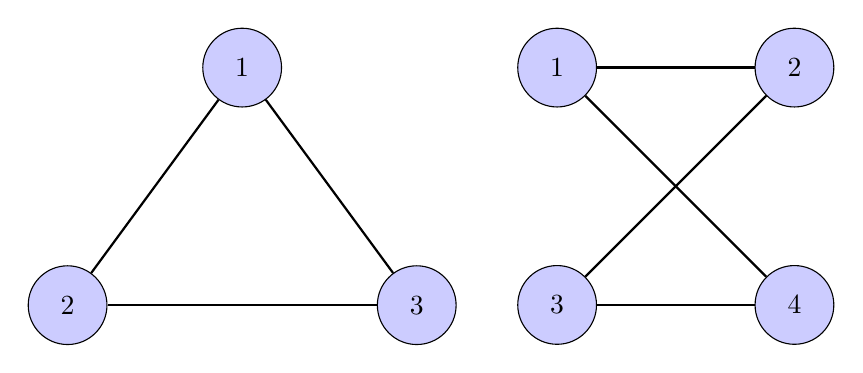
\begin{tikzpicture}
		\node[main node] (1) {$1$};
		\node[main node] (2) [below left = 2.3cm and 1.5cm of 1]  {$2$};
		\node[main node] (3) [below right = 2.3cm and 1.5cm of 1] {$3$};
		
		\path[draw,thick]
		(1) edge node {} (2)
		(2) edge node {} (3)
		(3) edge node {} (1);
		%%
		\begin{scope}[xshift=4cm]
			\node[main node] (1) {$1$};
			\node[main node] (2) [right = 2cm  of 1]  {$2$};
			\node[main node] (3) [below = 2cm  of 1] {$3$};
			\node[main node] (4) [right = 2cm  of 3] {$4$};
			
			\path[draw,thick]
			(1) edge node {} (2)
			(1) edge node {} (4)
			(3) edge node {} (2)
			(3) edge node {} (4)
			;
		\end{scope}
	\end{tikzpicture}
\caption{Egyszer\H u gr\'af TIKZ seg\'its\'eg\'evel}
\end{figure}



\newpage
\section {Saját szoftverek esetén}

Saját szoftverek esetében sikerült négy különböző technológia segítségével megvalósítani a Dorman-Prince differenciálegyenlet megoldó algoritmust (lásd \ref{fejezet3_2}. alfejezet). A felhasznált technológiák: Matlab, Java, C++ és Android voltak.

Ezen technológiák közül az Androidos szoftverrel kapcsolatban már előzetes félelmeink voltak, mivel azt feltételeztük, hogy bármennyire is fejlettek napjainkban a mobileszközök, mégis hardveresen nem lesznek elegek ahhoz, hogy versenybe tudjanak szállni a számítógépekkel. Néhány teszt után feltételezéseink beigazolódtak, láthatjuk a \ref{fejezet3_3}. alfejezet teszteseteiben is, hogy az Android szoftver mennyire gyengén teljesített (mind a Motorola Moto E2, mind a Samsung Galaxy Core Prime esetében). Összehasonlítva a többi algoritmussal az átlagidőket nézve $ 150-160 $ - szor lassabb a Javanál és $ 300 - 350 $ - szer a C++ - nál! Tehát azt a következtetést vonhatjuk le, hogy nem érdemes mobileszközökön differenciálegyenleteket oldani, mivel túlságosan nagy a hardver igénye és egyelőre ezen a téren nem képesek tartani a lépést a számítógépekkel.

A további három technológia közül (Matlab, Java, C++) meglepő módon itt is a Matlab teljesített a legjobban, igaz, hogy ebben az esetben már nem használtuk az ode45 programot, hanem megírtam én a saját függvényemet. Ez a teljesítményen is meglátszott, mert az általam írt függvény nem tudott jobban teljesíteni a tesztek alatt, mint az ode45. Mindezek ellenére $ 35-40 $ - szer gyorsabb volt a Javanál és megközelítőleg $ 15-20 $ - szor gyorsabb a C++ - nál.

A Java és C++ szoftvereket összehasonlítva elmondhatom, hogy az esetek többségében a C++ körülbelül $ 2 $ - szer volt gyorsabb a Javanál, ami megfelel az előzetes elvárásoknak.

Amit nagyon fontosnak tartok kihangsúlyozni, hogy az általam megvalósított C++ szoftver a tesztek során nagyon jól teljesített, felvette a versenyt az Odeint könyvtárral és az elért átlagok is csak nagyon kicsivel maradnak el az Odeint által produkált eredményektől (\ref{fejezet3_3}. alfejezet).

Továbbá megvalósítottam az Euler és Runge-Kutta módszerek párhuzamosított változatait is CUDA technológia segítségével. Ebben az esetben a tesztek azt mutatták, hogy az Euler módszer esetében többe kerül a sok CPU és GPU memória közötti másolás művelete, mint amennyit nyerünk a számítások elvégzése során. Tehát ebben az esetben ez a fajta párhuzamosítási megközelítés nem éri meg. Ezzel ellentétben a Runge-Kutta módszer esetében a megközelítés eredményesnek bizonyult abban az esetben, ha az egyenletek száma nagy és a lépésköz kicsi. A \ref{fejezet3_4} alfejezetben láthattuk, hogy abban az esetben ha az egyenletek száma $ n = 10 $ és a lépésköz $ h = 0.001 $, a GPU-n megközelítőleg 5 és fél perccel hamarabb lefutott az algoritmus, mint a CPU-n. Ezzel a párhuzamosítási módszerrel nem tudtuk kihasználni a videókártya által nyújtott maximális számítási kapacitást, de így is jelentős különbséget sikerült elérni a futási időket nézve, l\'asd \cite{Katai}.



\section {Összességében}

A fentieket összegezve elmondhatom, hogy megéri előre megírt szoftvereket vagy könyvtárakat használni differenciálegyenletek megoldására. Nagyon megkönnyíthetik az eltünket egyszerűségükkel és nagy teljesítményükkel. Viszont fontos elmondani, hogy használatuk problémákkal is járhat, például fizetni kell értük vagy nem lehet belenyúlni az algoritmusokba kedvünk szerint, esetleges fellépő hibák esetén nagyon nehéz lenyomozni a hiba forrását (vagy szinten lehetetlen).

Saját algoritmusok terén bátran elmondhatom, hogy megéri a C++ technológiát választani és ezen a vonalon továbbhaladni egy esetleges saját könyvtár megírása, megvalósítása felé. Láthattuk, hogy az általam megírt C++ szoftver is felvette a versenyt az Odeint könyvtárral, ami szintén C++ technológiát alkalmaz, l\'asd \cite{Antal}.

Egy másik vonal, amit érdemes sokkal jobban felderíteni az a CUDA technológiával és grafikus kártyával történő differenciálegyenlet megoldása. Láthattuk, hogy egy kis párhuzamosítás is jelentős időbeli különbséget jelenthet bizonyos algoritmusok esetében. Annak tudatában is, hogy a differenciálegyenletek megoldása nem a legjobban adatpárhuzamosítható feladatok közé sorolható azt mondom, hogy megéri ezzel a technológiával foglalkozni. Ennek kapcsán a legnagyobb motiváció számomra a jövőre nézve a parciális differenciálegyenletek párhuzamosításának megvalósítása és tanulmányozása, mivel ezeknél az egyenleteknél jobban ki lehet használni a videókártya rácsos szerkezetét.
	%----------------------------------------------------------------------------
\chapter{Tervezés és megvalósítás}
%----------------------------------------------------------------------------

A rendszer architektúrájának tervezése során figyelembe vettem a \ref{research}. és \ref{scopes}. fejezetekben kitűzött célokat. Az eredeti tervek elkészültével kezdetét vette a megvalósítás. Az implementáció során felmerültek olyan akadályok és újabb ötletek, amelyek kisebb-nagyobb mértékben befolyásolták a terveket. Erre számítottam és éppen ezért úgy próbáltam tervezni, hogy dinamikusan módosíthatóak legyenek bővítés vagy módosítás esetén. A tervezési és megvalósítási folyamat hónapokat vedd igénybe annak érdekében, hogy minden jelentkező problémát és az újabb ötleteket legyen idő átgondolni.

\section {Az alkalmazás frontendje}

\subsection {Kezdőoldal (Homepage)}

Tekintettel arra, hogy az alkalmazás bizonyos funkcionalitásai használhatóak bejelentkezés nélkül is, a kezdőoldal egy üdvözlő oldal egy navigációs menüvel az oldal tetején. Amennyiben egy eszközről első alkalommal lépik az oldalra egy felhasználó, akkor egy információs ablakkal találkozik \cite{Modal}, amely tartalmazza az alkalmazás célját, a hivatalos forrásokat a jegyvásárlásra és ezeknek a jogtulajdonosait (\ref{abra:homepagePopup}).

Annak érdekében, hogy ez az ablak csak egyszer jelenjen meg \textbf{sütiket (Cookies)} használok. Ezek a sütiket a böngésző tárolja a felhasználó eszközén és a weboldal betöltésekor a böngésző betölti az elmentett sütiket, ha vannak. Ezek kulcs-elem párok, amely értelmében egy tetszőleges nevű kulcs alatt tudok elmenteni majdnem bármilyen adatot. Ha a felhasználó rákattint az \textbf{Understood} gombra, akkor egy \textbf{modalAccepted} kulcs alatti sütiben eltárolom a \textbf{true} értéket és amikor betöltődik az alkalmazás ezt az értéket ellenőrzöm.
Mint említettem ezek a sütik lokálisan vannak tárolva a felhasználónál és ha a felhasználó kitörli azokat, amelyek ehhez az oldalhoz tartoznak, akkor egyértelműen újra elő fog jönni az ablak.

\begin{figure}[!h]
	\centering
	\includegraphics[scale=0.4]{images/homepagePopup}
	\caption{Kezdőoldalon felugró ablak}
	\label{abra:homepagePopup}
\end{figure}
\pagebreak

\begin{figure}[!h]
	\centering
	\includegraphics[scale=0.2]{images/homepage}
	\caption{Kezdőoldal}
	\label{abra:homepage}
\end{figure}
\pagebreak

\subsection {Versenynaptár (Schedule)}

A \textbf{Versenynaptár} oldalon lehet böngészni a 2022-es év versenyeinek listáját a megrendezési sorrendben. Az első kártya, ami megjelenik az oldalon az a következő verseny, amely automatikusan kerül ki az aktuális dátum alapján. Teszt jelleggel van egy dátum kiválasztó gomb is, hogy ki lehessen próbálni, hogy egy adott dátumhoz melyik verseny lesz a legközelebb. Erre a kártyára kattintva meg lehet tekinteni a részleteket. Minden kártyán látszanak a legfontosabb információk az adott versenyről, mint a pálya neve, a rendező ország neve, az intervallum, amikor az esemény zajlani fog és a pályarajz (\ref{abra:schedule}). Továbbfejlesztési lehetőség, hogy csak azok a pályák legyenek aktívak, amelyek még hátra vannak.

\begin{figure}[!h]
	\centering
	\begin{tabular}{cc}
	\includegraphics[scale=0.15]{images/schedule1} &
	\includegraphics[scale=0.15]{images/schedule2} \\
	A versenynaptár & Görgetéssel látható az összes pálya
	\end{tabular}
	\caption{Versenynaptár}
	\label{abra:schedule}
\end{figure}

Ha átvisszük az egeret a kártya fölott, akkor megjelenik egy gomb \textbf{Browse tickets} szöveggel, amelyre kattintva megtekinthetőek a versenyhez tartozó jegy típusok és azok információi (\ref{abra:ticketsUA}). Ha nincs bejelentkezve a felhasználó, akkor az \textbf{Add to cart} gomb szürkén jelenik meg, vagyis nem lehet a kosárba tenni, viszont ha rákattint a felhasználó, akkor a rendszer jelezni fogja egy \textbf{alert} (figyelmeztetés) ablakban, hogy autentikáció szükséges, ha ezt a funkciót szeretné használni.

\begin{figure}[!h]
	\centering
	\includegraphics[scale=0.2]{images/tickets}
	\caption{Jegy típusok be nem jelentkezett felhasználóval}
	\label{abra:ticketsUA}
\end{figure}

Abban az esetben, ha a felhasználó be van jelentkezve, lehetőség van a jegyet a kosárba helyezni. Egy továbbfejlesztési lehetőség, hogy visszajelzést tudjon adni az adott jegyről, élményekről (\ref{abra:ticketsAuth}). A jegyek mennyiségét a \textbf{Checkout} oldalon van lehetősége módosítani a felhasználónak. A rendszer ezen része egy továbbfejlesztési terület, hogy adott esetben ellenőrizve legyen, hogy tényleg csak az tudjon visszajelzést adni, akkor vásárolt az adott jegyből. 

\begin{figure}[!h]
	\centering
	\includegraphics[scale=0.2]{images/ticketsAuth}
	\caption{Jegy típusok bejelentkezett felhasználóval}
	\label{abra:ticketsAuth}
\end{figure}

\subsection {Bejelentkezés és regisztráció (Sign in and up)}

A bejelentkezési felületen egyben lett feltüntetve a bejelentkezés és regisztráció két külön kártyán. Az email címmel vagy közösségi fiókkal való autentikáción kívül lehetőség van elfelejtett jelszó esetén új megadása. Ennek érdekében a felhasználó megadja az email címét és kapni fog egy levelet, amely tartalmaz egy linket az új jelszó megadásához (\ref{abra:signInUp}).

\begin{figure}[!h]
	\centering
	\includegraphics[scale=0.2]{images/signInUp}
	\caption{Autentikáció}
	\label{abra:signInUp}
\end{figure}

Továbbá lehetőség van a felületre való regisztrációra is a jobb oldali kártyán. Ennek a folyamatnak a bemutatására készítettem egy szekvencia diagramot a \textbf{SequenceDiagram.org} online szerkesztő segítségével \cite{Seq}.

\begin{figure}[!h]
	\centering
	\includegraphics[scale=0.5]{images/signUpFlow}
	\caption{Szekvencia diagram - Regisztráció}
	\label{abra:signUpFlow}
\end{figure}
\pagebreak

A regisztráció folyamatát a felhasználó indítja el a kötelező mezők kitöltésével. A \textit{Firebase} szerver első sorban ellenőrzi, hogy az adott email címmel már létezik-e felhasználó és amennyiben igen, a megfelelő üzenetet jeleníti meg az oldal. Ellenkező esetben létrehozza a rendszerben a felhasználót, elmenti a megadott adatokat egyéb meta adatokkal kiegészítve, mint a létrehozás dátuma. A mentés után a rendszer automatikusan be is jelentkezteti a felhasználót (\ref{abra:signUpFlow}).

\subsection {Profil (Profile)}

A \textbf{Profil} oldal elérése csak a bejelentkezett felhasználóval lehetséges (\ref{abra:profile}). Ezen az oldalon lehetséges a profilkép és a megjelenített név módosítása az \textbf{Edit profile} gombra kattintva.

\begin{figure}[!h]
	\centering
	\includegraphics[scale=0.2]{images/profile}
	\caption{Saját profil oldal}
	\label{abra:profile}
\end{figure}

Az oldal jobb részén láthatóak a \textbf{rendelési előzmények}. Ezek görgetéssel böngészhetőek és a jobb szélén levő ikonra kattintva tekinthetőek meg a vásárlás részletei (\ref{abra:previousOrders}).

\begin{figure}[!h]
	\centering
	\includegraphics[scale=0.3]{images/previousOrders}
	\caption{Rendelés részletei}
	\label{abra:previousOrders}
\end{figure}

Amennyiben elvisszük valamely elem fölött az egeret megjelenik egy \textbf{More details} gomb, amelyre kattintva megtekinthető a jegy egyedi azonosítója (\ref{abra:moreDetails}). Ez a funkcionalitás azért fontos, mivel megtörténhet, hogy a felhasználó elveszíti vagy nem kapja meg a QR kódot emailben, ami ezt az azonosítót tartalmazza. Ha ez bekövetkezne, akkor innen is lehetőség van kimásolni és a megszokott módon azonosítani a PIN kóddal.

Ezen a felugró ablakon továbbá lehetősége van a felhasználónak egy új PIN kódot megadni, ha az aktuálist elfelejtette vagy úgy érzi, hogy valaki megszerezhette. Ezután egy újabb felugró ablakban lehetséges a PIN kód megváltoztatása. 

\begin{figure}[!h]
	\centering
	\includegraphics[scale=0.4]{images/moreDetails}
	\caption{Jegy részletei}
	\label{abra:moreDetails}
\end{figure}

A PIN kód megadásánál kötelezően egy 6 számjegyű számot kell megadni (\ref{abra:pinPopup}). Ezt manuálisan is be lehet írni vagy a \textit{pálca} ikonra kattintva generálódik egy véletlenszerű szám. A \textbf{Submit} gombra kattintva frissítheti a felhasználó a jegyhez tartozó kódot, ami teljes mértékben felülírja az előzőt, ezért nagyon figyelmes kell lenni a megadásakor, de erre a pirossal írt szöveg is figyelmezteti a vásárlót.

\begin{figure}[!h]
	\centering
	\includegraphics[scale=0.4]{images/pinPopup}
	\caption{PIN kód megadása}
	\label{abra:pinPopup}
\end{figure}
\pagebreak

\subsection {Rendelés (Checkout)}

A \textbf{Rendelés} oldalon van lehetősége a felhasználónak véglegesíteni a vásárlást (\ref{abra:checkout}). Itt is láthatóak a kosárba helyezett jegyek információi és csak itt módosíthatóak az egyes jegyek mennyisége vagy a kosárból való törlése. A \textbf{Pay Now} gombra kattintva a felhasználó meg tudja adni a számlázási adatokat majd a kártyaadatokat a vásárlás véglegesítéséhez. Ezt a \textbf{Stripe} szolgáltatás segítségével valósítottam meg. Sikeres vásárlás esetén a felhasználónak küld a rendszer egy emailt, amiben megkapja a QR kódokat. Egy kód tartalmazza a rendelés egyedi azonosítóját kombinálva a felhasználó egyedi azonosítójával. Az emailek küldésére a \textbf{Brevo} szolgáltatót vettem igénybe \cite{Brevo}.

\begin{figure}[!h]
	\centering
	\includegraphics[scale=0.2]{images/checkout}
	\caption{Rendelés véglegesítése}
	\label{abra:checkout}
\end{figure}

A rendelés leadása után az adatok eltárolására használt titkosítás elvégzésére több megoldást is kipróbáltam, amelyek közül az egyik az \ref{code:encryption} kódrészlet, amely az AES algoritmus egyik használati módja JavaScript programozási nyelven a CryptoJS könyvtárcsomag segítségével.

A kód első lépése a \textit{salt (só)} generálása, ami egy 128/8 bájt szekvencia, amely segítségével meghatározásra kerül majd a key (kulcs). A \textit{CryptoJS.lib.WordArray.random(128 / 8)} kódsor a \textbf{CryptoJS} könyvtárban található \textit{random()} függvény hívásával egy véletlenszerű 128-bites szekvenciát generál, majd beilleszti az adatokat a WordArray osztályba.

A következő lépésben a kulcs előállítása történik meg a \textit{secretPass (jelszó)} és a só használatával a kulcsderiváló függvény segítségével. A kulcs előállítása a \textit{CryptoJS.PBKDF2()} függvénnyel történik, amely egy kulcstervező függvény. Az első paraméter a titkosításhoz használt jelszó, a második argumentum a só, a harmadik pedig a kulcs hosszát és az iterációk számát határozza meg. Ennél az algoritmusnál nagyon fontos odafigyelni, hogy a jelszó szigorúan titkos információ, vagyis ezt biztonságosan ajánlott eltárolni szerver oldalon. A többi paraméter publikus, mert önmagukban nem elegendőek a titkosított szöveg visszafejtéséhez.

Az inicializáló \textit{vektor (iv)} generálása következik. Az IV egy véletlenszerű bájt szekvencia, amelynek hossza megegyezik a blokk méretével (128 bit), és a titkosítás során használják, hogy azonos adatok esetén is véletlenszerű kimenetet generáljon.

Az adat titkosítása a \textit{CryptoJS.AES.encrypt()} függvénnyel történik. Az adatot először JSON formátumba alakítjuk, majd az AES algoritmust a kulcs, az IV és további paraméterek (mód, padding és tag) megadásával alkalmazzuk. A \textit{mode} a blokktitkosítási mód (BCM) kiválasztására szolgál, ezek között található a ECB, CBC, OFB vagy CFB. A mi esetünkben a CBC (Cipher Block Chaining) mód van használva.

\begin{lstlisting}[caption={Titkosítás példakód.}, captionpos=b, language = JavaScript, label={code:encryption}]
export const encryptData = text => {
  const salt = CryptoJS.lib.WordArray.random(128 / 8);
  const key = CryptoJS.PBKDF2(secretPass, salt, {
    keySize: 256 / 32,
    iterations: 1000,
  });
  const iv = CryptoJS.lib.WordArray.random(128 / 8);

  const encrypted = CryptoJS.AES.encrypt(JSON.stringify(text), key, {
    iv: iv,
    mode: CryptoJS.mode.CBC,
    padding: CryptoJS.pad.Pkcs7,
    tag: true,
  });

  const data = {
    ciphertext: encrypted.ciphertext.toString(CryptoJS.enc.Base64),
    iv: iv.toString(CryptoJS.enc.Base64),
    salt: salt.toString(CryptoJS.enc.Base64),
    tag: true,
  };
  return JSON.stringify(data);
};
\end{lstlisting}

A \textit{padding} a blokkok kitöltési módját határozza meg, itt a \textbf{Pkcs7} (Public Key Cryptography Standards 7-es szabványa) van használva. A Pkcs7 padding szabvány szerint, ha az üzenet hossza nem egész blokk méretű, akkor azt szükséges kiegészíteni. Minden hiányzó bájt felveszi a hiányzó bájtok számának megfelelő értéket. Ha például az utolsó blokkban 3 hiányzó bájt van, akkor a blokk utolsó bájtjai a 0x03 értéket veszi fel.

Az \textit{iv} az inicializáló vektort tartalmazza, amit korábban generáltunk. A \textit{tag} beállítása igazra van állítva, hogy az üzenet hitelesítése (integritásának ellenőrzése) is megtörténjen a titkosítás során. A tag az üzenet elejére kerül beillesztésre a titkosítás során, és végül az eredeti üzenet végén kerül ellenőrzésre a helyessége.

Az utolsó lépés a \textit{titkosított adat (ciphertext)}, az IV, a só és az üzenet hitelesítésének értéke (tag) összekapcsolása és JSON formátumba rendezése és visszatérítése.

Az alábbi példakód a visszafejtést valósítja meg (\ref{code:decryption}):

\begin{lstlisting}[caption={Visszafejtés példakód.}, captionpos=b, language = JavaScript, label={code:decryption}]
export const decryptData = text => {
const json = JSON.parse(text);
const salt = CryptoJS.enc.Base64.parse(json.salt);
const iv = CryptoJS.enc.Base64.parse(json.iv);
const tag = json.tag;
const ciphertext = CryptoJS.enc.Base64.parse(json.ciphertext);

const key = CryptoJS.PBKDF2(secretPass, salt, {
	keySize: 256 / 32,
    	iterations: 1000,
});

const decrypted = CryptoJS.AES.decrypt(
  	{ ciphertext: ciphertext, salt: salt, iv: iv, tag: tag },
    	key,
    	{
     	iv: iv,
      	mode: CryptoJS.mode.CBC,
      	padding: CryptoJS.pad.Pkcs7,
      	tag: true,
    }
  );
  return JSON.parse(decrypted.toString(CryptoJS.enc.Utf8));
};
\end{lstlisting}

A \textbf{decrypt} függvény az \textbf{encrypt} függvénnyel ellentétes sorrendben dolgozza fel az adatokat. A paraméterként kapott titkosított szövegből JSON objektumot állít elő. Ezután ebből az objektumból megkapja a só és az iv Base64 formátumból az értékeket. A kulcs előállítása a \textit{PBKDF2} függvénnyel történik a jelszó és a só segítségével. A titkosított adat, az iv, a só és a hitelesítési tag felhasználásával sikeresen vissza tudjuk fejteni az eredeti üzenetet.

A másik opció a \textbf{CryptoJS} csomag mellett a \textbf{node-rsa} könyvtárcsomag segítségével megvalósított titkosítás és RSA kulcscsere volt \textbf{NodeJS} keretrendszerben. A \ref{code:rsaEncrypt} kódrészletben az adat titkosítása látható a RSA publikus kulcs segítségével (\ref{code:rsaGenrerate} kódrészlet), amelyet minden rendelés során a rendszer generál a privát kulcs mellett. A titkosítás során szükség van a \textit{publicKey}-re, amely a generálás során elmentődik az adatbázisba és ezt lekéri a rendszer. A publicKey segítségével titkosítom az \textit{AES} kulcsot, amellyel titkosítom az eredeti szöveget. A végeredmény egy \textbf{encryptedData} és egy \textbf{encryptedKey} lesz, amelyek hasonlóan bekerülnek az adatbázisba az összesített rendelések közé, az \textbf{orders} dokumentumba.

\begin{lstlisting}[caption={RSA kulcscsere és titkosítás.}, captionpos=b, language = JavaScript, label={code:rsaEncrypt}]
const aesKey = CryptoJS.lib.WordArray.random(16).toString();
const encryptedData = CryptoJS.AES
	.encrypt(<unique code with PIN code>, aesKey).toString();

const rsaKey = new NodeRSA();
rsaKey.importKey(publicKey, "public");
const encryptedKey = rsaKey.encrypt(aesKey.toString(), "base64");
\end{lstlisting}

\begin{lstlisting}[caption={RSA kulcsok generálása.}, captionpos=b, language = JavaScript, label={code:rsaGenrerate}]
const key = new NodeRSA({ b: 2048 });
const publicKey = key.exportKey("public");
const privateKey = key.exportKey("private");
\end{lstlisting}

A \ref{code:rsaDecrypt} kódrészletben lekéri a rendszer a rendeléshez tartozó privát kulcsot, majd annak segítségével visszafejti a titkosított \textit{AES} kulcsot. Ezzel a kulccsal már vissza lehet fejteni a titkosított szöveget, ezáltal megkapni a az eredeti szöveget az egyedi azonosítóval és a PIN kóddal.

\begin{lstlisting}[caption={RSA visszafejtés.}, captionpos=b, language = JavaScript, label={code:rsaDecrypt}]
const rsaKey = new NodeRSA();
rsaKey.importKey(privateKey, "private");
const decryptedKey = rsaKey.decrypt(data?.encryptedKey, "utf8");

const decryptedData = CryptoJS.AES.decrypt(
	data?.encryptedData,
	decryptedKey
).toString(CryptoJS.enc.Utf8);
\end{lstlisting}

\pagebreak
\subsection {Beléptetés (Scan)}

A \textbf{Beléptetés} oldalon a rendszer \textit{Adminisztrátora(i)} tudják a jegyeket hitelesíteni a versenyhelyszíneken az erre a célra kihelyezett termináloknál (\ref{abra:scan}). A felhasználó a kamera elé helyezi a QR kódot \cite{RQR}, majd beírja a PIN kódot, amelyeket a rendszer rögzít és jelzi a hitelesítési folyamat eredményét.

\begin{figure}[!h]
	\centering
	\includegraphics[scale=0.2]{images/scan}
	\caption{Jegyek hitelesítése}
	\label{abra:scan}
\end{figure}
	%%----------------------------------------------------------------------------
\chapter{Szoftver}
%----------------------------------------------------------------------------

\section {A szoftver bemutatása}

\section {Diagramok}

\subsection{Use Case diagram}

\subsection{Osztálydiagram}
	
\subsection{Szekvencia diagram}
	%----------------------------------------------------------------------------
\chapter*{Összefoglaló}\addcontentsline{toc}{chapter}{Összefoglaló}
%----------------------------------------------------------------------------

Dolgozatomban differenciálegyenletek megoldásával foglalkoztam, amelyet különböző programozási technológiák segítségével valósítottam meg. Először ismertettem a differenciálegyenletek numerikus megoldásának elméleti alapjait, majd megvizsgáltunk és levezettünk három numerikus módszert az Euler-, a Runge-Kutta és a Dormand-Prince módszereket. Ezek közül a mai technológiákban leginkább használatos Dormand-Prince algoritmus esetében megnéztük, hogy milyen szoftverekben tálálhatjuk meg, mint alapértelmezett differenciálegyenlet megoldó. A továbbiakban ismertettem két modellt, a leukémia betegség alap modelljét és a hullámmozgás modelljét, ezzel is kihangsúlyozva a téma fontosságát, hogy mennyire fontos az időtényező bizonyos problémák egyenleteinek medoldásánál. Ezek után részletesen is mégnéztük, hogy milyen szoftvereket alkalmaztam és alkottam a differenciálegyenletek és rendszerek megoldására. A szoftvereket két kategóriába osztotottuk fel, az első a már létező szoftverek kategóriája, a másik pedig az általam megvalósított szoftverek csoportja volt. Az első kategóriában ismertettem két technológiát, a Matlab által nyúltott ode45 beépített megoldót és a Boost könyvtárcsomagban található Odeint nevű könyvtárat. Az általam írt szofverek csoportjában négy megvalósítást mutattam be ezek a Matlab, Java, C++ és Android technológiák segítségével készültek. Emellett megnéztük, hogy mennyire hatékonyan lehet párhuzamosítani a differenciálegyenletek megoldását CUDA technológia segítségével és a grafikus kártyát (GPU-t) felhasználva. Végül kiértékeltük a tesztelés során kapott eredményeket és összehasonlítottuk a különböző programokat, kiemelve azok erősségeit és gyengéit. Majd levontuk a következtetéseket, hogy melyik technológia irányában érdemes tovább haladni és melyik az, amelyikkel nem éri meg foglalkozni.

Jövőbeli terveimet illetően szeretnék jobban elmerülni a GPU-n történő differenciálegyenletek megoldásának módszereiben, valamint ezek alkalmazását kipróbálni és tanulmányozni a parciális differenciálegyenletek területén (PDE). Továbbá érdemesnek tartom a C++ szoftver továbbfejlesztését és egy differenciálegyenlet megoldó könyvtár megalkotását, amely ingyenesen használható és nyílt forráskódú lenne.

% Koszonetnyilvanitas
%~~~~~~~~~~~~~~~~~~~~~~~~~~~~~~~~~~~~~~~~~~~~~~~~~~~~~~~~~~~~~~~~~~~~~~~~~~~~~~~~~~~~~~
	%\include{acknowledgement}
	%----------------------------------------------------------------------------
\addcontentsline{toc}{chapter}{Jelölések}
%----------------------------------------------------------------------------
\chapter*{Jelölések}

\begin{table}[h!]
	\centering
	\begin{tabular}{ | l | c | c | c | c |}
		\hline 
		\textbf{Rövidítés} & \textbf{Angol megnevezés} & \textbf{Magyar megnevezés}\\
		\hline
		F1 & Formula One & Formula-1/Forma-1\\
		\hline
		FIA & International Automobile Federation & Nemzetközi Automobil Szövetség \\
		\hline
		F1TM & F1 Ticket Manager & - \\
		\hline
		EDI & Electronic Data Interchange & Elektronikus Adatcsere \\
		\hline
		PDF & Portable Document Format & Hordozható Dokumentum Formátum \\
		\hline
		QR Code & Quick Response Code & Quick Response-kód (=gyors válasz) \\
		\hline
		E2EE & End-To-End Encryption & Végpontok Közötti Titkosítás \\
		\hline
		PIN & Postal Index Number & Postai Indexszám \\
		\hline
		DOM & Document Object Model & Dokumentum Objektum Modell \\
		\hline
		OSS & Open-Source Software & Nyílt Forráskódú Szoftver \\
		\hline
		NoSQL & Not only Structured Query Language & Nem csak Strukturált
		 Lekérdezőnyelv \\
		\hline
		API & Application Programming Interface & Alkalmazásprogramozási Felület \\
		\hline
		CDN & Content Delivery Network & Tartalomelosztó Hálózat \\
		\hline
		IDE & Integrated Development Environment & Integrált Fejlesztői Környezet \\
		\hline
		DBMS & Database Management Systems & Adatbázis-kezelő Rendszer (ABKR) \\
		\hline
		UI & User Interface & Felhasználói Felület \\
		\hline
		UX & User Experience & Felhasználói Élmény \\
		\hline
		HTML & HyperText Markup Language & Hiperszöveges Jelölőnyelv \\
		\hline
		CSS & Cascading Style Sheets & Lépcsőzetes Stíluslapok \\
		\hline
		HTTP & HyperText Transfer Protocol & Hiperszöveges Szállítási Protokoll \\
		\hline
		BCM & Block Cipher Mode & Blokktitkosítási Mód \\
		\hline
		AES & Advanced Encryption Standard & - \\
		\hline
		RSA & Rivest–Shamir–Adleman & - \\
		\hline
		REST & Representational State Transfer & - \\
		\hline
		MIT & Massachusetts Institute of Technology & Massachusettsi Műszaki Egyetem \\
		\hline
		\end{tabular}
		\label{tablazat1}
\end{table}


% Tablazatok es abrak jegyzeke (EZ NEM KOTELEZO)
%~~~~~~~~~~~~~~~~~~~~~~~~~~~~~~~~~~~~~~~~~~~~~~~~~~~~~~~~~~~~~~~~~~~~~~~~~~~~~~~~~~~~~~
	\listoffigures\addcontentsline{toc}{chapter}{\abrakjegyzeke}
	%\listoftables\addcontentsline{toc}{chapter}{\tablazatokjegyzeke}


% Bibliography
%~~~~~~~~~~~~~~~~~~~~~~~~~~~~~~~~~~~~~~~~~~~~~~~~~~~~~~~~~~~~~~~~~~~~~~~~~~~~~~~~~~~~~~
	\bibliography{mybib}
	\addcontentsline{toc}{chapter}{\irodalomjegyzek}
	\bibliographystyle{alpha}
	
% Appendix
%~~~~~~~~~~~~~~~~~~~~~~~~~~~~~~~~~~~~~~~~~~~~~~~~~~~~~~~~~~~~~~~~~~~~~~~~~~~~~~~~~~~~~~
	%\include{appendices}

\label{page:last}
\end{document}
